\documentclass[conference]{article}
\usepackage{cite}
\usepackage{amsmath,amssymb,amsfonts}
\usepackage{algorithm}
\usepackage{algpseudocode}
\algblock{ParFor}{EndParFor}
% customising the new block
\algnewcommand\algorithmicparfor{\textbf{for}}
\algnewcommand\algorithmicpardo{\textbf{do in parallel}}
\algnewcommand\algorithmicendparfor{\textbf{end parallel for}}
\algrenewtext{ParFor}[1]{\algorithmicparfor\ #1\ \algorithmicpardo}
\algrenewtext{EndParFor}{\algorithmicendparfor}
\usepackage{float}
\usepackage{graphicx}
\usepackage[table,xcdraw]{xcolor}
\usepackage{textcomp}
\usepackage{markdown}
\usepackage{subcaption}
\usepackage{placeins}
\usepackage{graphics}
\usepackage{hyperref}
\usepackage{multirow}
\usepackage{array}
\usepackage{listings}
 \usepackage{color}
 \definecolor{codegreen}{rgb}{0,0.5,0.0}
\definecolor{codegray}{rgb}{0.5,0.5,0.5}
\definecolor{codepurple}{rgb}{0.58,0,0.82}
\definecolor{backcolour}{rgb}{0.95,0.95,0.92}

\newcommand{\beginsupplement}{%
        \setcounter{table}{0}
        \renewcommand{\thetable}{S\arabic{table}}%
        \setcounter{figure}{0}
        \renewcommand{\thefigure}{S\arabic{figure}}
        \setcounter{algorithm}{0}
        \renewcommand{\thealgorithm}{S\arabic{algorithm}}
     }

\beginsupplement

\newcommand*{\myfont}{\fontfamily{lmtt}\selectfont}
\newcommand*{\toolnamefont}{\fontfamily{lmdh}\selectfont}

\newcommand{\commentKhaled}[1]{\textbf{\color{red}{#1}}}

\newcommand{\toolname}{{BatchLayout}}
\newcommand{\toolnameBH}{{BatchLayoutBH}}
\date{}
\usepackage{xcolor}
\begin{document}
\setcounter{page}{1}
\title{BatchLayout: A Batch-Parallel Force-Directed Graph Layout Algorithm in Shared Memory\\ (supplementary file)}
\author{Md. Khaledur Rahman, Majedul Haque Sujon and Ariful Azad}
\maketitle
\section{Online Repository}
\toolname{} is publicly available at \url{https://github.com/khaled-rahman/BatchLayout}. Benchmark datasets, results and well-documented instructions also available in the repository. Note that we have also shared other tools and instructions about how to run. For OpenOrd, we have both Gephi's version and author's version.

\section{How to compile \toolname{}}
We will be continuing to improve performance \toolname{} using different optimization techniques such as vectorized operations which will be available at \url{https://github.com/khaled-rahman/BatchLayoutCode}. To compile our source code at \url{https://github.com/khaled-rahman/BatchLayout} without errors, users must have OpenMP version 4.5 and GCC version 4.9. We compiled and run it on linux and macOS. To compile source code, user can type following commads:\newline
\begin{markdown}
```
make clean;
make
```
\end{markdown}

\section{How to run \toolname{}}
Once you successfully compiled source code, type following commad to run \toolname{}:\newline
\begin{markdown}
```
./BatchLayout -input 3elt_dual.mtx -output output/ -iter 600 -batch 256 -threads 32 -algo 2
```
\end{markdown}

Here, parameters have following meaning: 
\newline
\begin{markdown}
```
-input <filename>, full path with file name.
```
\end{markdown}
\newline
\begin{markdown}
```
-output <dir>, output directory where layout is saved.
```
\end{markdown}
\newline
\begin{markdown}
```
-iter <int>, an integer indicates number of iteration. Detaulf:600.
```
\end{markdown}
\newline
\begin{markdown}
```
-batch <int>, an integer indicates size of batch. Default:256.
```
\end{markdown}
\newline
\begin{markdown}
```
-threads <int>, an integer indicates number of threads. Default is max number of threads available in the computing machine.
```
\end{markdown}
\newline
\begin{markdown}
```
-algo <int>, an integer among 0 to 6 which indicates a particular variation of BatchLayout. Default:2. 
```
\end{markdown}

\FloatBarrier
\begin{table*}[htbp]
\centering
\caption{Layouts of different graphs generated by different tools.}
\label{tab:layouts}

\begin{tabular}{|c|p{1.2cm}|p{1.4cm}|p{1.2cm}|p{1.4cm}|p{1.2cm}|p{1.2cm}|}
\hline
\textbf{Graph}   & \textbf{BL} & \textbf{BLBH} & \textbf{FA2} & \textbf{FA2BH} & \textbf{OOG} & \textbf{OO} \\ \hline
        \textbf{Powergrid} & \multicolumn{6}{|c|}{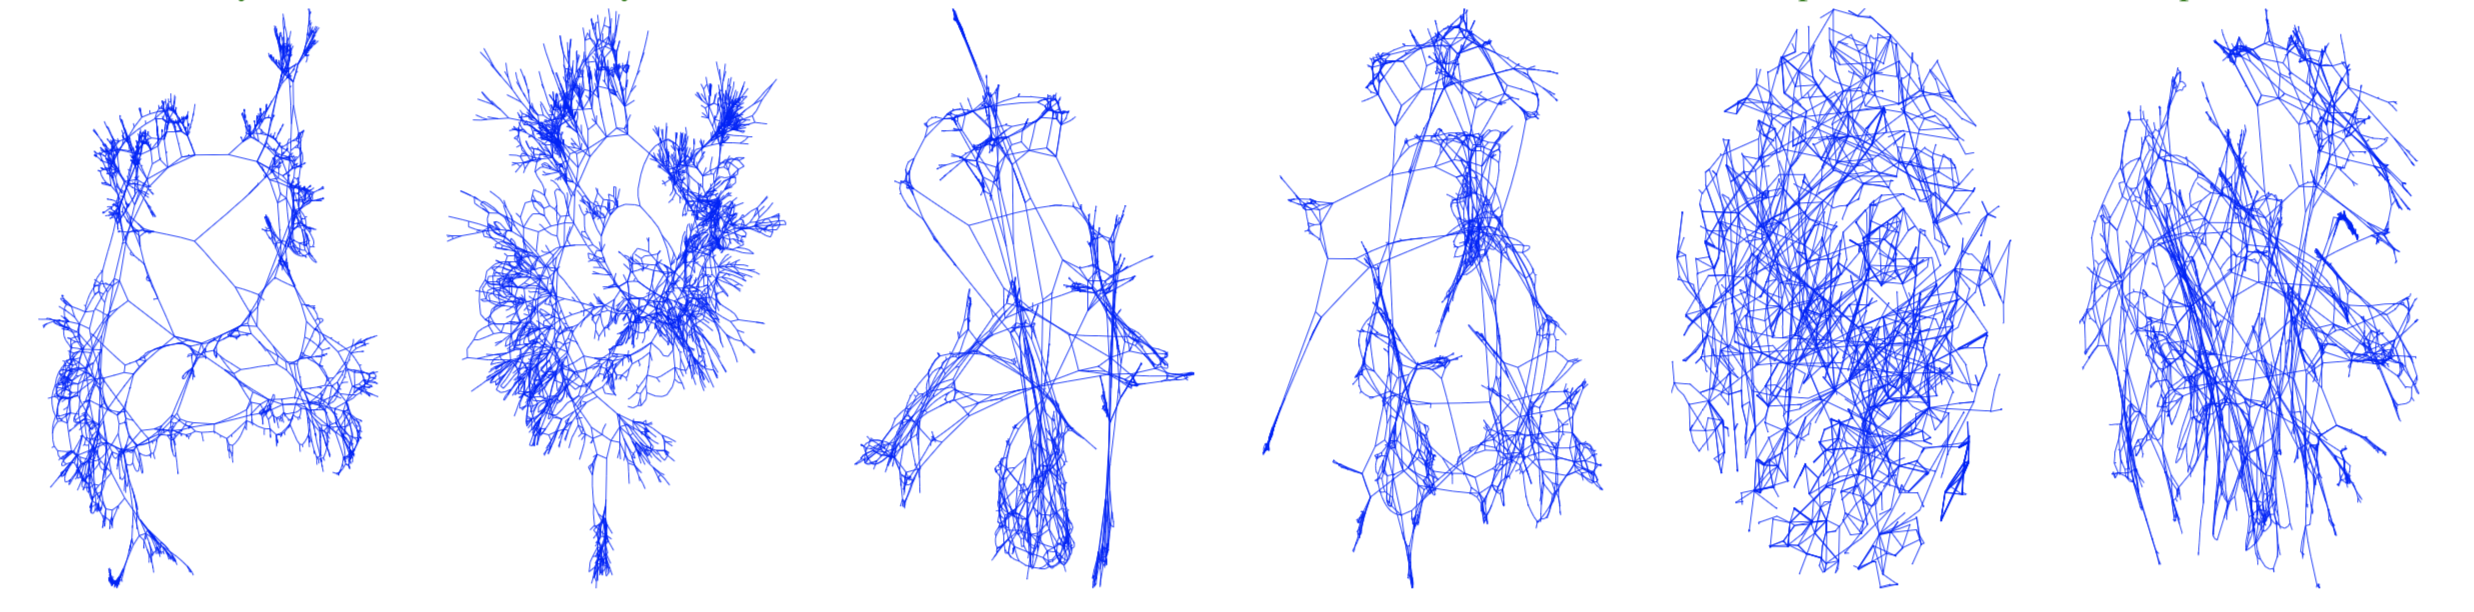
\includegraphics[height=2.05cm,width=0.8\linewidth]{layouts/powernetwork.png}}                                                                                                                \\ \hline
\textbf{add32}   & \multicolumn{6}{c|}{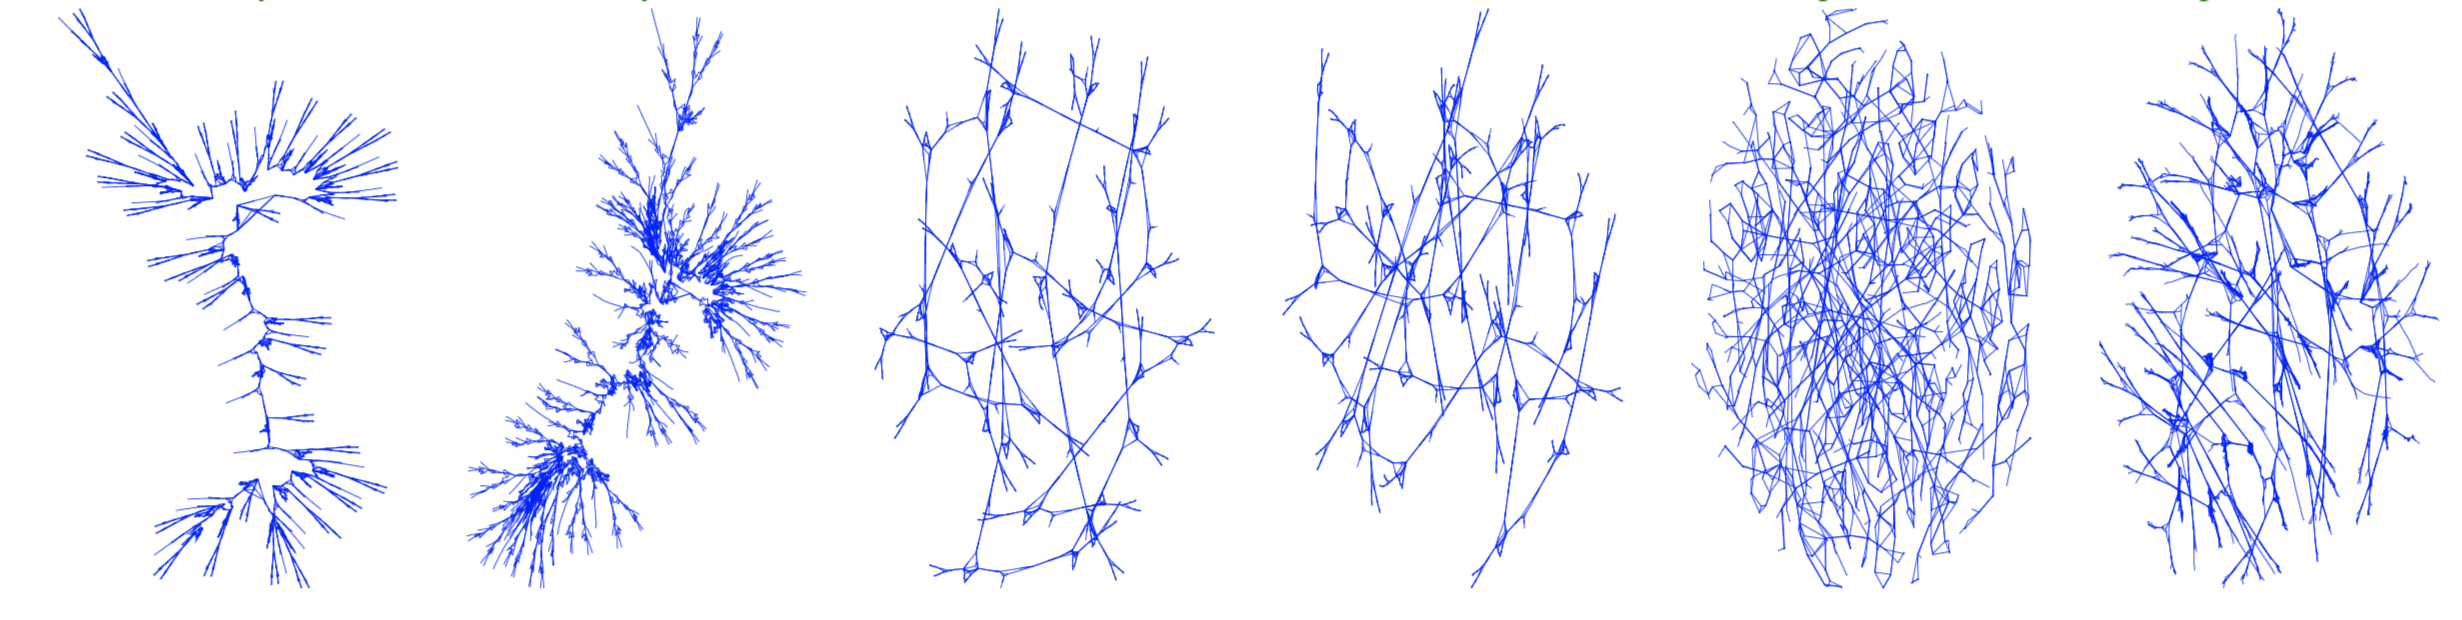
\includegraphics[height=2.05cm,width=0.8\linewidth]{layouts/add32.png}}                                                                                                                 \\ \hline
\textbf{ba\_network}        & \multicolumn{6}{c|}{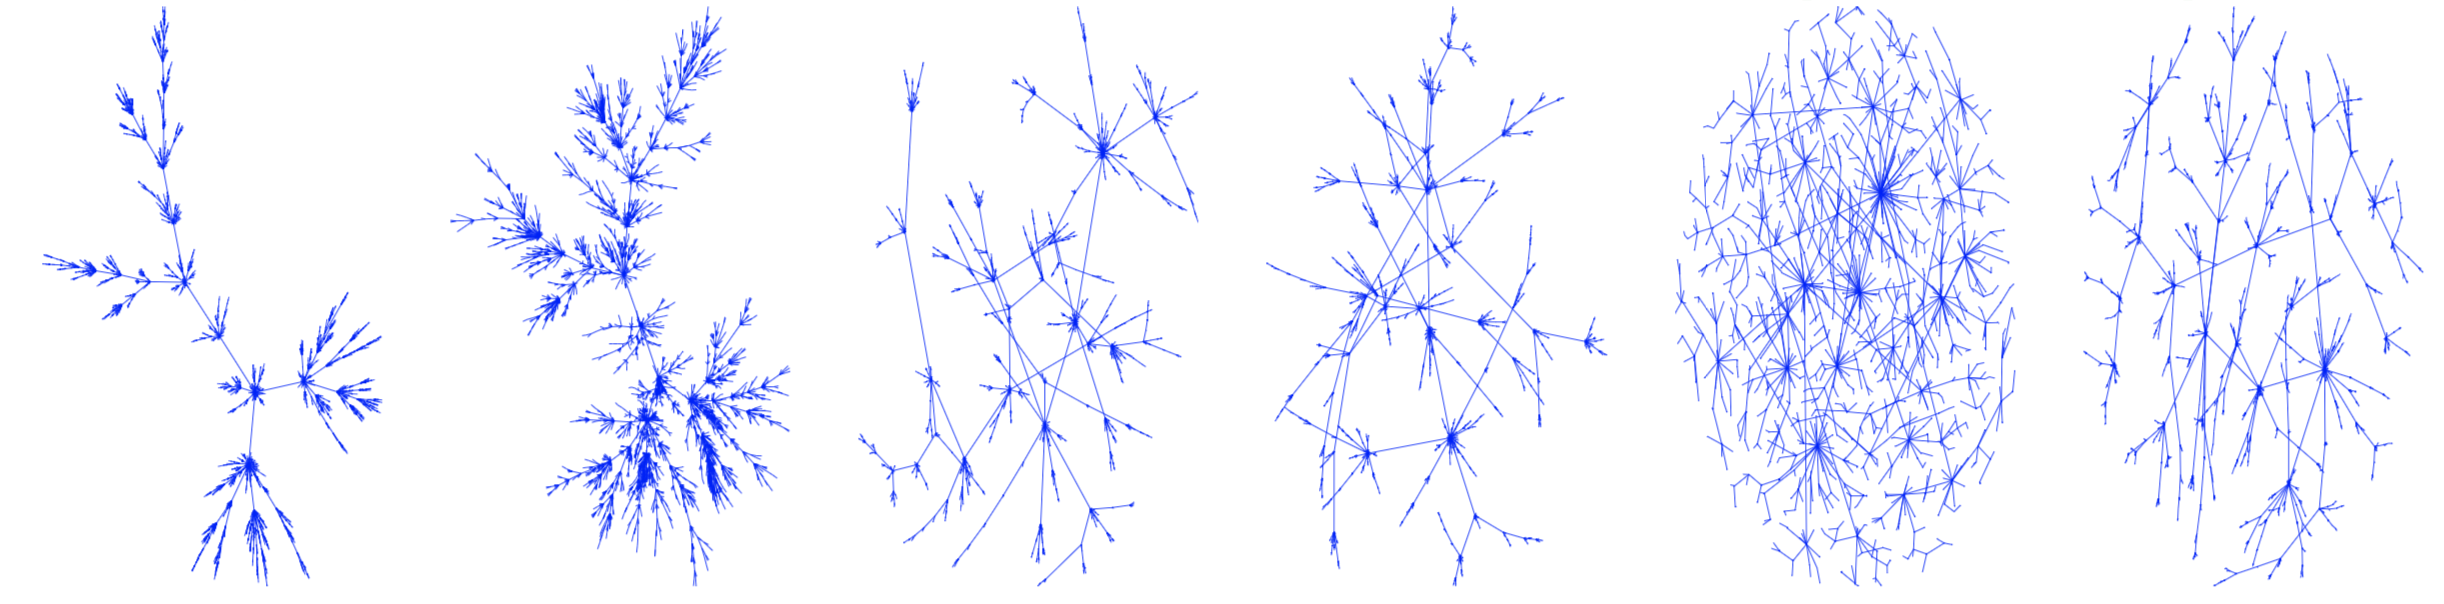
\includegraphics[height=2.05cm,width=0.8\linewidth]{layouts/sf_6000.png}}                                                                                                                 \\ \hline
\textbf{3elt\_dual}        & \multicolumn{6}{c|}{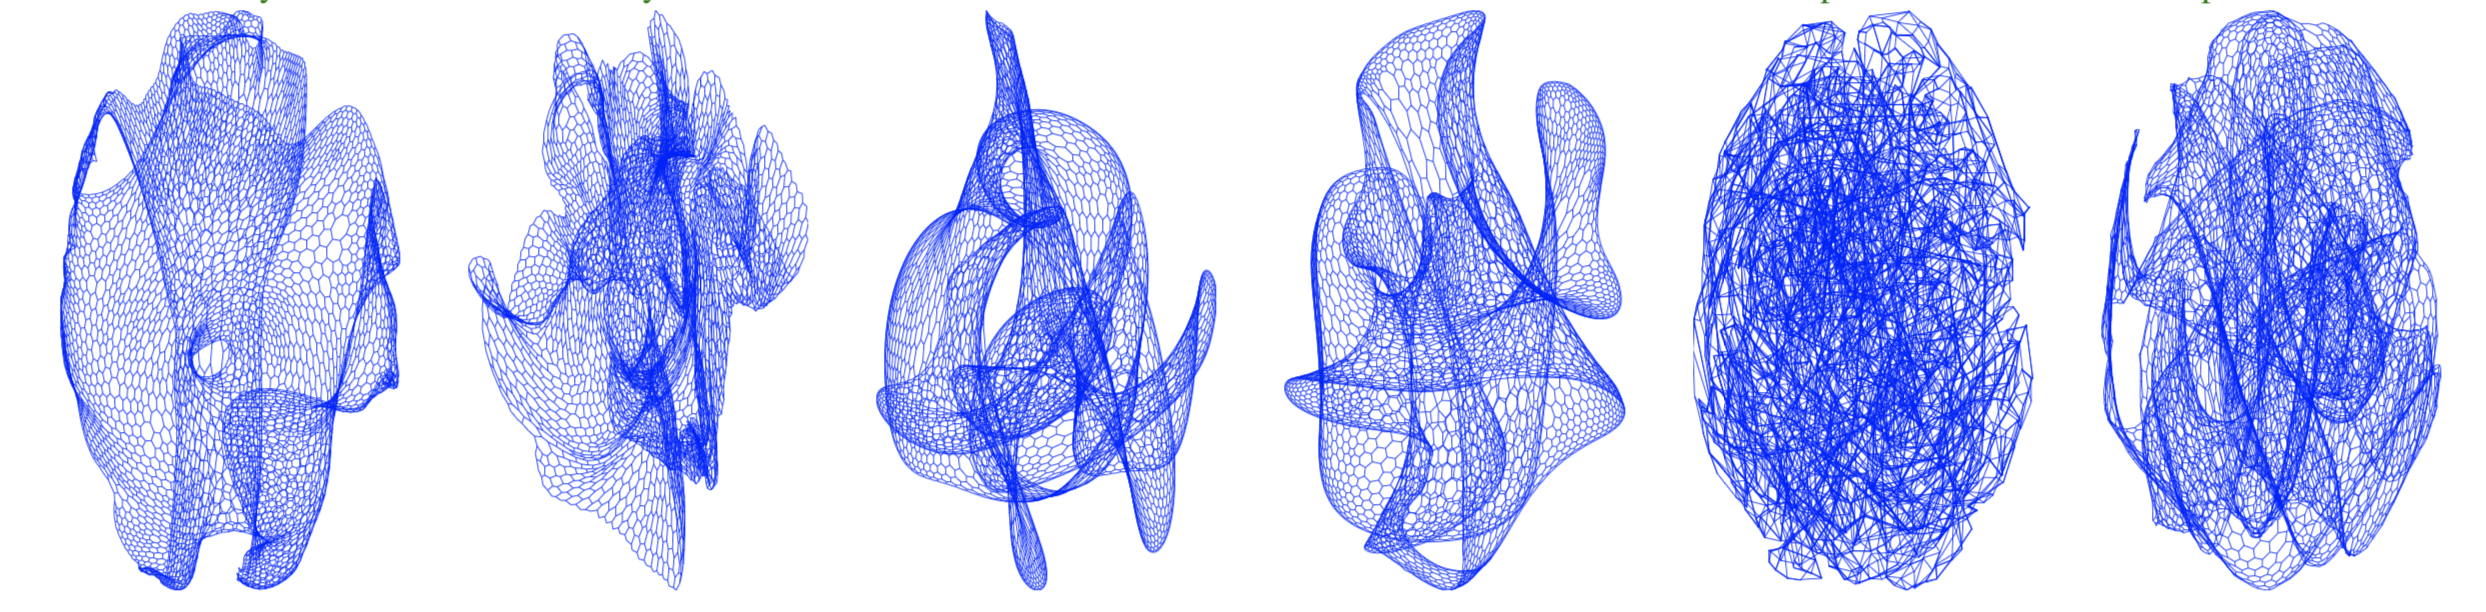
\includegraphics[height=2.05cm,width=0.8\linewidth]{layouts/3elt_dual.png}}                                                                                                                 \\ \hline
\textbf{PGPgiant.}        & \multicolumn{6}{c|}{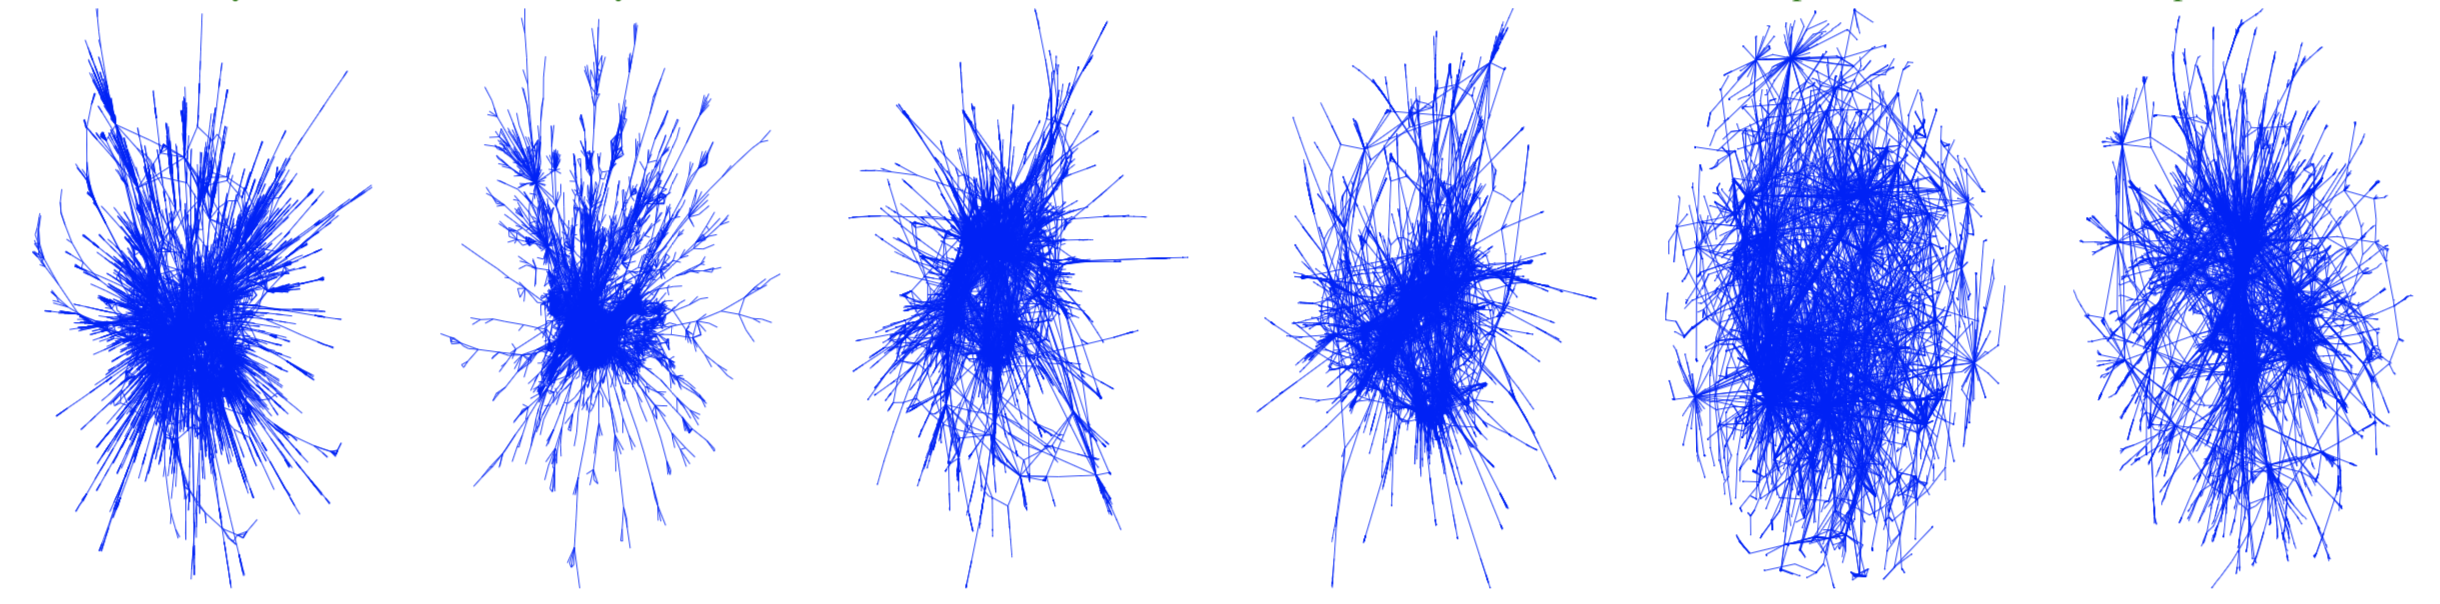
\includegraphics[height=2.05cm,width=0.8\linewidth]{layouts/PGPgiantcompo.png}}                                                                                                                 \\ \hline
\textbf{pkustk02}        & \multicolumn{6}{c|}{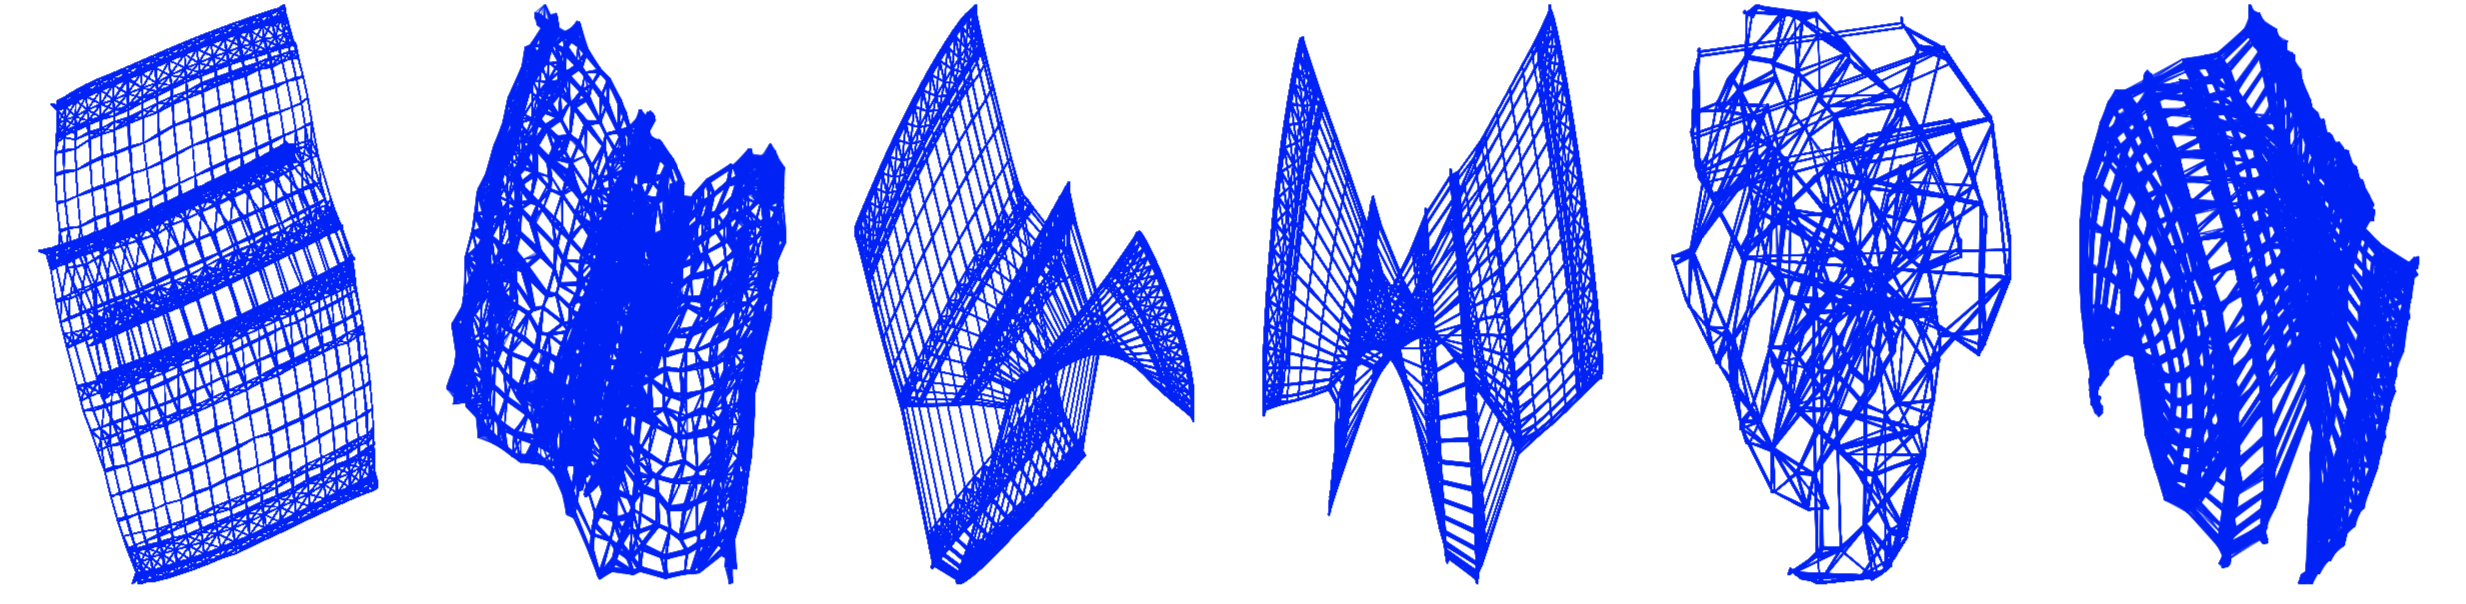
\includegraphics[height=2.05cm,width=0.8\linewidth]{layouts/pkustk02.png}}                                                                                                                 \\ \hline
\textbf{fe\_4elt2}        & \multicolumn{6}{c|}{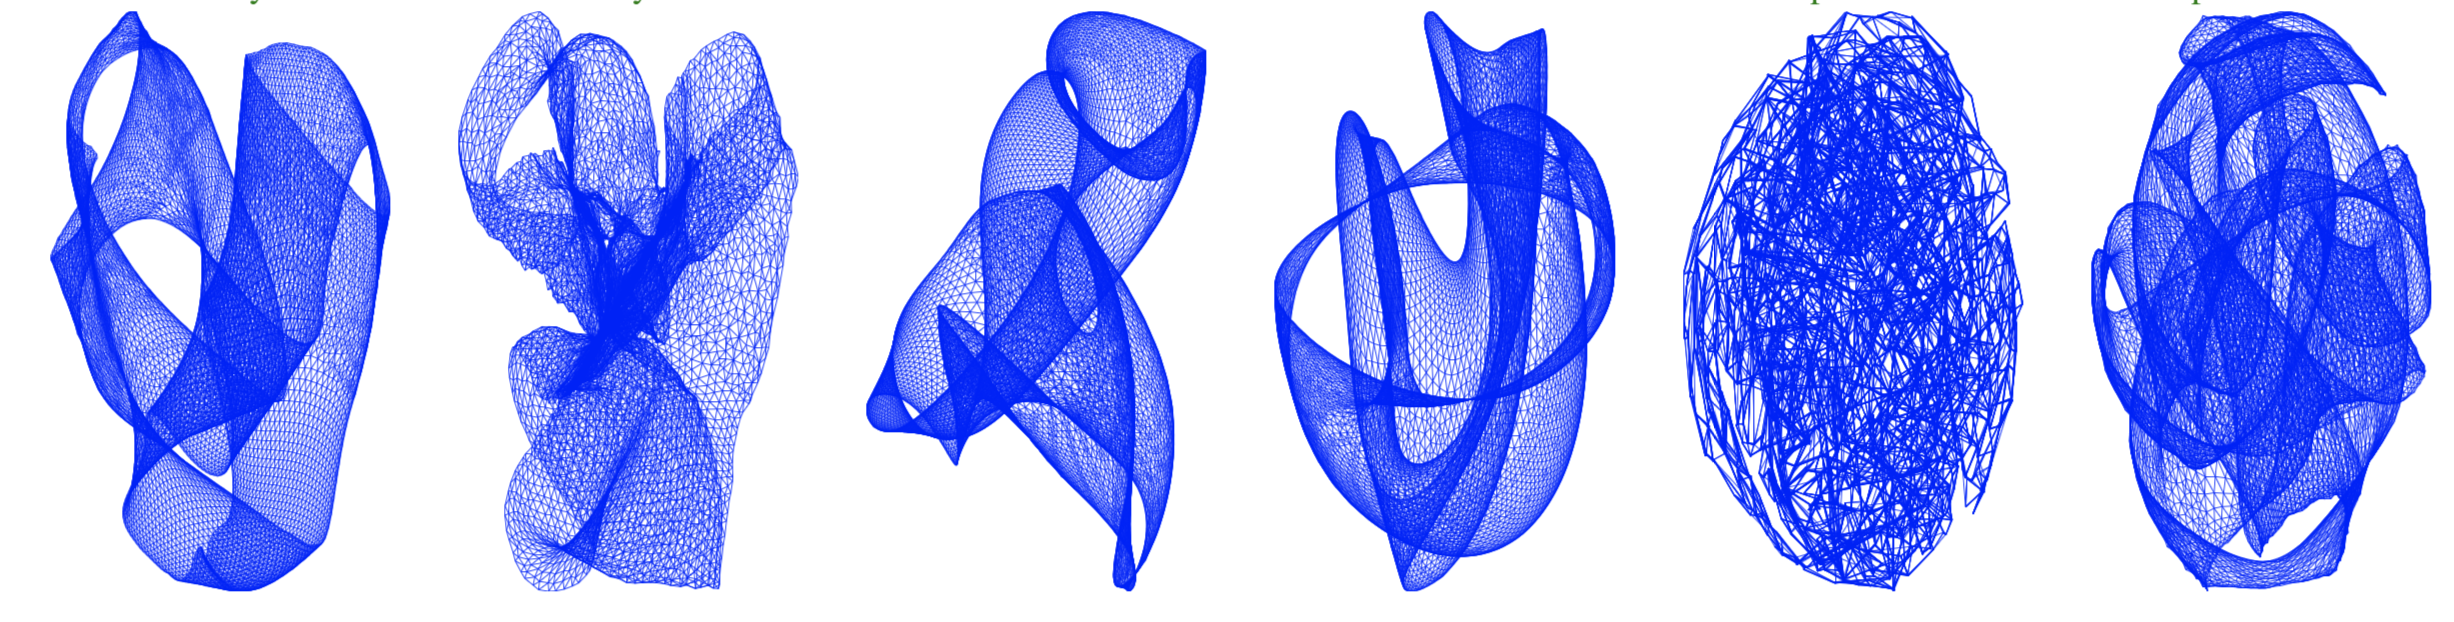
\includegraphics[height=2.05cm,width=0.8\linewidth]{layouts/fe_4elt2.png}}                                                                                                                 \\ \hline
\textbf{bodyy6}        & \multicolumn{6}{c|}{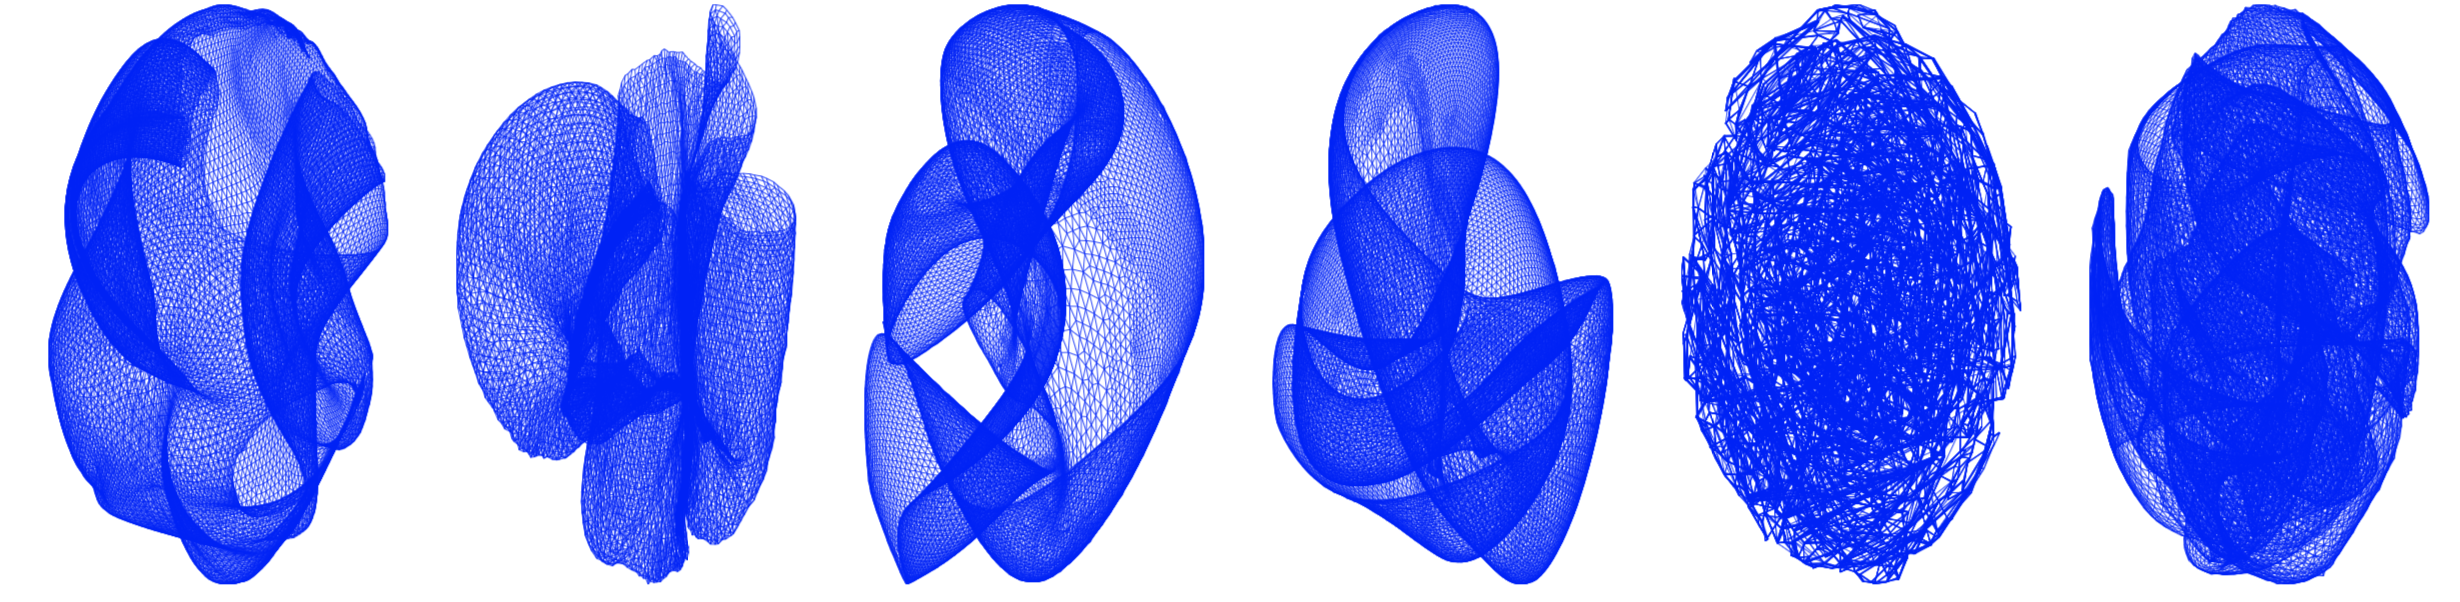
\includegraphics[height=2.05cm,width=0.8\linewidth]{layouts/bodyy6.png}}                                                                                                                 \\ \hline

\textbf{pkustk01}        & \multicolumn{6}{c|}{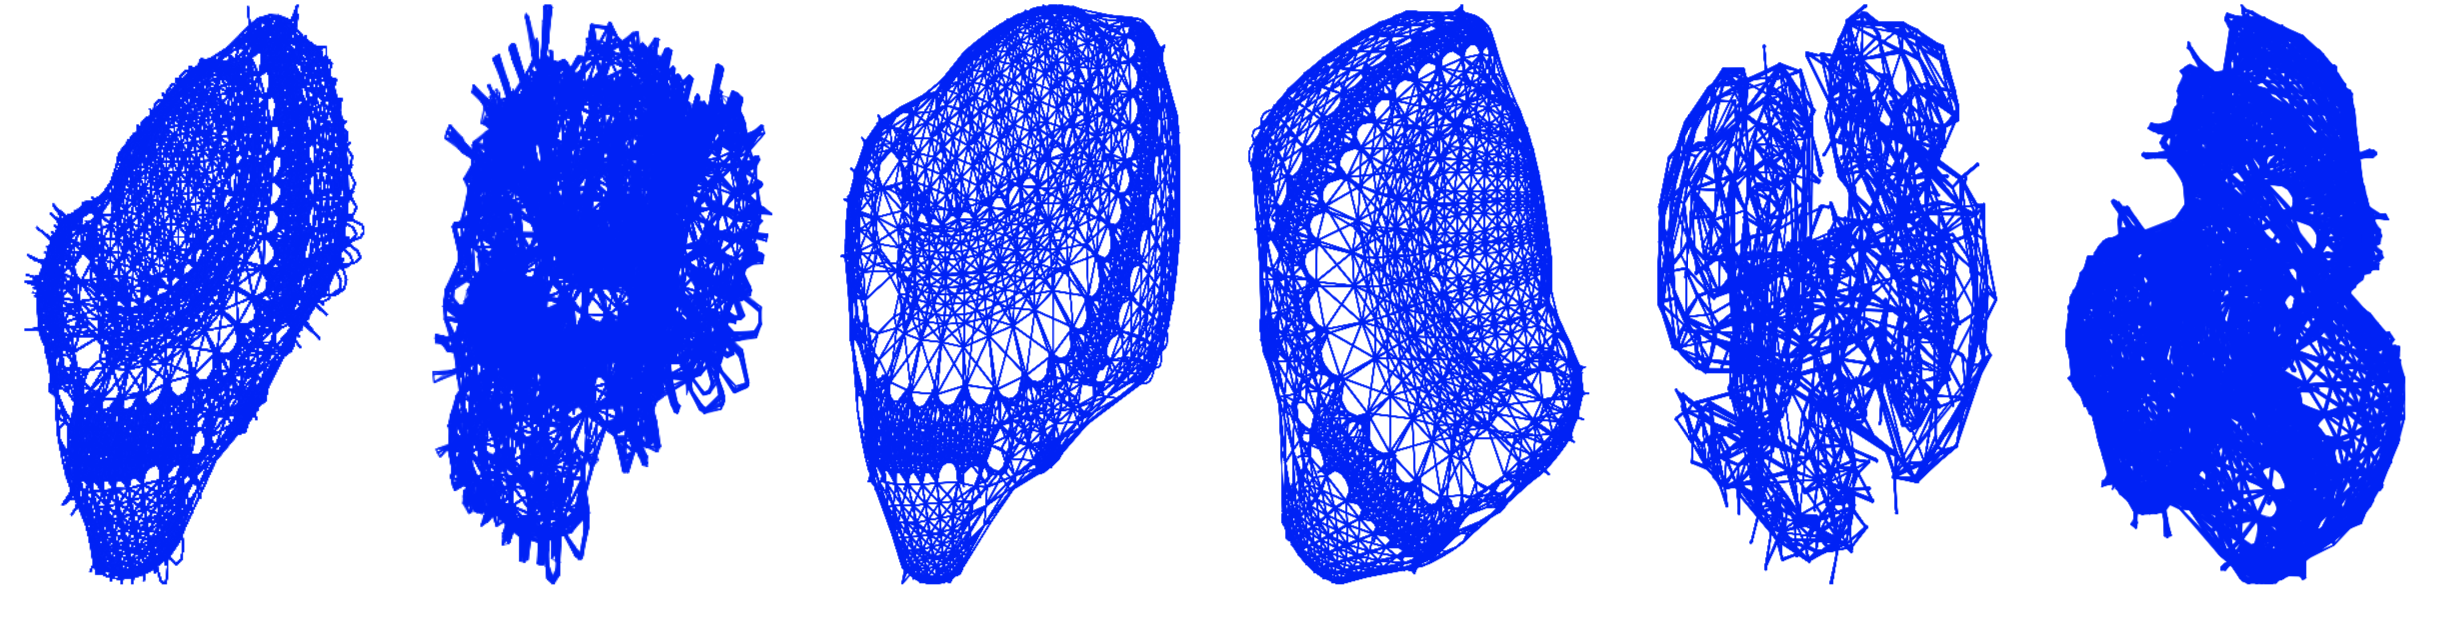
\includegraphics[height=2.05cm,width=0.8\linewidth]{layouts/pkustk01.png}}  \\ \hline

\end{tabular}
\end{table*}

% Please add the following required packages to your document preamble:
% 
% If you use beamer only pass "xcolor=table" option, i.e. \documentclass[xcolor=table]{beamer}
\begin{table}[!htb]
\caption{Convergence of BatchLayout for a threshold value of 1E-6 and values of `Iteration' and `Energy' are for converged layouts. Running time in seconds for other tools for corresponding number of iterations that BatchLayout takes to converged.}
\centering
\label{tab:contime}
\begin{tabular}{|c|c|c|
>{\columncolor[HTML]{C0C0C0}}c |
>{\columncolor[HTML]{C0C0C0}}c |
>{\columncolor[HTML]{C0C0C0}}c |
>{\columncolor[HTML]{C0C0C0}}c |
>{\columncolor[HTML]{C0C0C0}}c |}
\hline
\textbf{Graph} & \textbf{Iter.} & \textbf{Energy} & \textbf{BL} & \textbf{FA2} & \textbf{OO} & \textbf{BLBH}  & \textbf{FA2BH} \\ \hline
power\_grid    & 12445                 & 0.036              & \textbf{26.95}   & 553.25            & 31.83                 & 26.99          & 65.32          \\ \hline
ba\_network    & 9216                  & 13.92              & 28.71            & 461.92            & 29                    & \textbf{23.7}  & 59.69          \\ \hline
3elt\_dual     & 1410                  & 1.3E6           & 8.58             & 160.29            & 6.99                  & \textbf{4.21}  & 13.18          \\ \hline
pkustk02       & 1792                  & 2.9E7           & 15.95            & 377.17            & 12.75                 & \textbf{7.52}  & 40.8           \\ \hline
fe\_4elt2      & 3590                  & 298895             & 32.33            & 591.76            & 21.66                 & \textbf{11.99} & 42.92          \\ \hline
bodyy6         & 2042                  & 7.5E6           & 52.2             & 708.63            & 21.51                 & \textbf{11.15} & 39.58          \\ \hline
pkustk01       & 8995                  & 35.853             & 305.49           & 5231.91           & 119.67                & \textbf{72}    & 305.11         \\ \hline
finance256     & 3747                  & 8.5E6           & 354.43           & 4846.48           & 75.19                 & \textbf{40.19} & 152.44         \\ \hline
\end{tabular}
\end{table}


\begin{table}[!htp]
\caption{Distribution of loops for OpenOrd tool used in Table \ref{tab:contime}}
\centering
\begin{tabular}{|c|c|c|c|c|c|c|}
\hline
\textbf{OpenOrd} & \textbf{25\%} & \textbf{25\%} & \textbf{25\%} & \textbf{10\%} & \textbf{15\%} & \textbf{total 100\%} \\ \hline
power\_grid      & 3111          & 3111          & 3111          & 1245          & 1867          & 12445                \\ \hline
ba\_network      & 2304          & 2304          & 2304          & 922           & 1382          & 9216                 \\ \hline
3elt\_dual       & 353           & 353           & 353           & 141           & 210           & 1410                 \\ \hline
pkustk02         & 448           & 448           & 448           & 179           & 269           & 1792                 \\ \hline
fe\_4elt2        & 898           & 898           & 898           & 359           & 537           & 3590                 \\ \hline
bodyy6           & 511           & 511           & 511           & 204           & 305           & 2042                 \\ \hline
pkustk01         & 2249          & 2249          & 2249          & 900           & 1348          & 8995                 \\ \hline
finance256       & 937           & 937           & 937           & 375           & 561           & 3747                 \\ \hline

\end{tabular}
\end{table}


\begin{table}[!htp]
\centering
\caption{Layouts of \emph{3elt\_dual.mtx} graph generated by BatchLayout for different iterations and batches. BS - batch size. Number in each column represents number of iteration and each row represents size of a batch.}
\label{tab:gridlayout}

\begin{tabular}{|p{1.7cm}|p{1.3cm}|p{1.3cm}|p{1.3cm}|p{1.3cm}|p{1.3cm}|p{1.3cm}|}
\hline
\textbf{}   & \textbf{300} & \textbf{600} & \textbf{900} & \textbf{1200} & \textbf{1500} & \textbf{1800} \\ \hline
        \textbf{BS=1} & \multicolumn{6}{|c|}{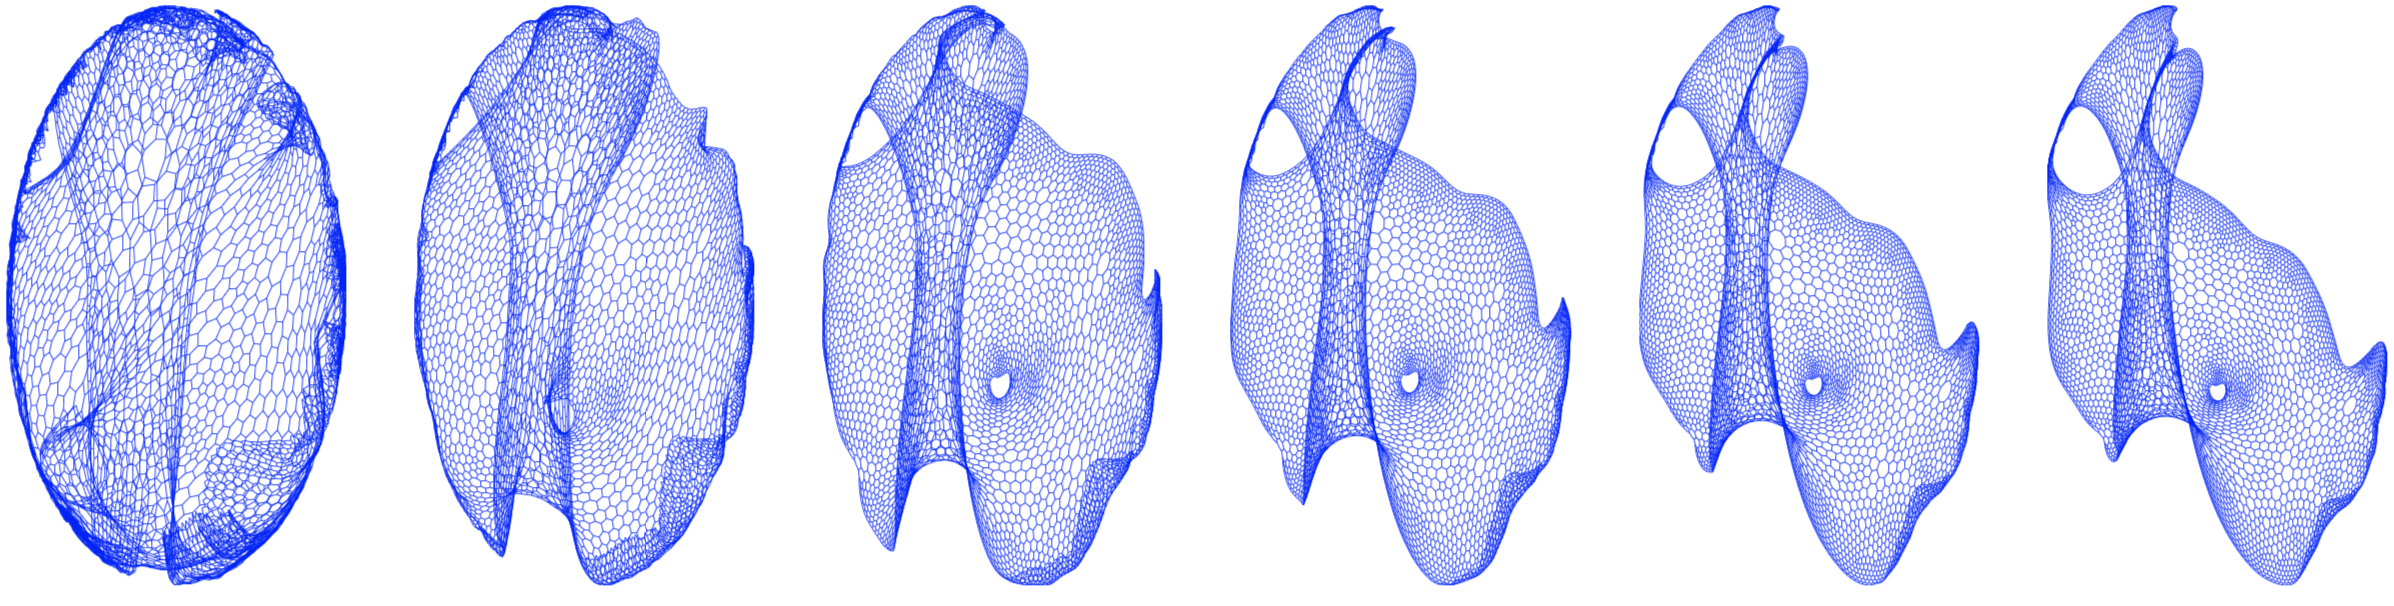
\includegraphics[height=2.2cm,width=0.8\linewidth]{layouts/batches/batch1.png}}                                                                                                                \\ \hline

    \textbf{BS=8} & \multicolumn{6}{|c|}{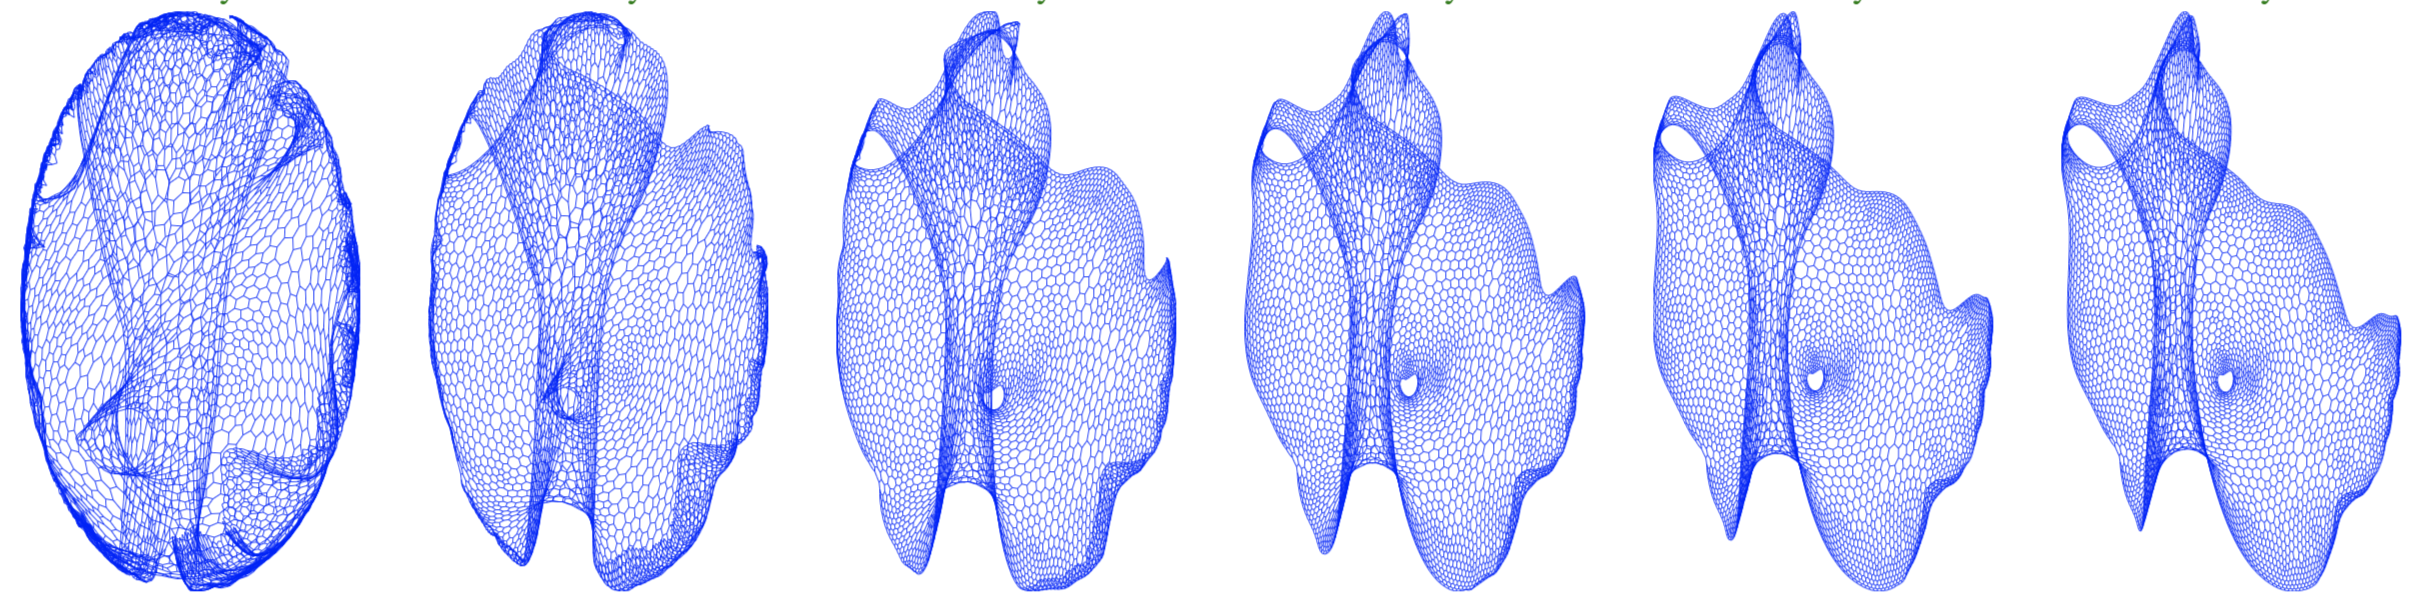
\includegraphics[height=2.2cm,width=0.8\linewidth]{layouts/batches/batch8.png}}                                                                                                                \\ \hline
    
            \textbf{BS=64} & \multicolumn{6}{|c|}{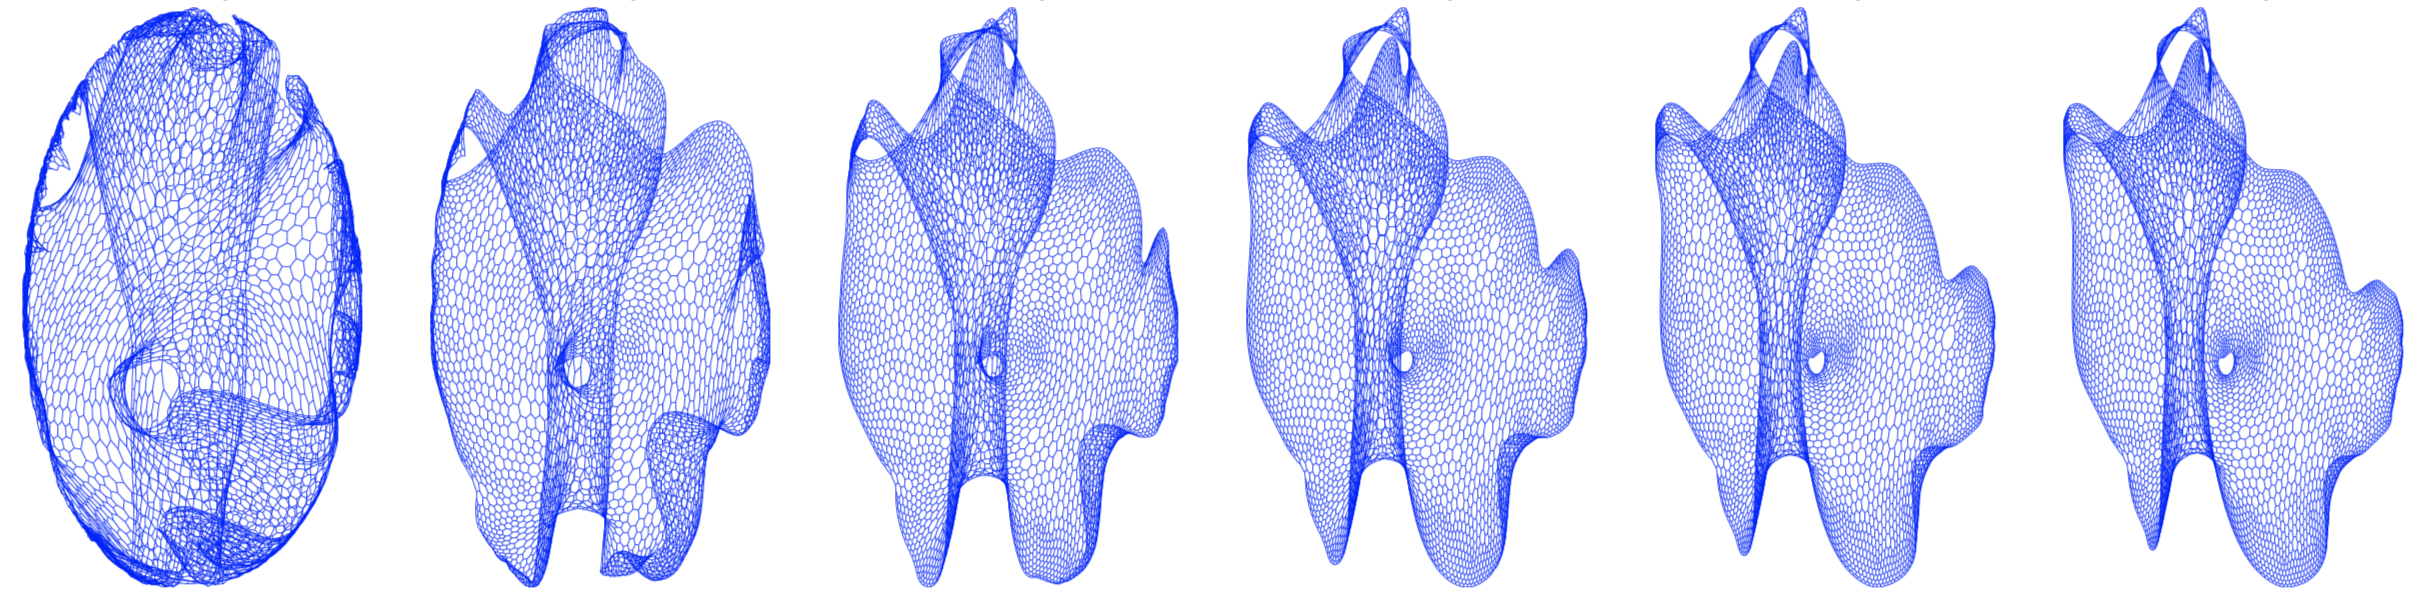
\includegraphics[height=2.2cm,width=0.8\linewidth]{layouts/batches/batch64.png}}                            \\ \hline
            
            \textbf{BS=256} & \multicolumn{6}{|c|}{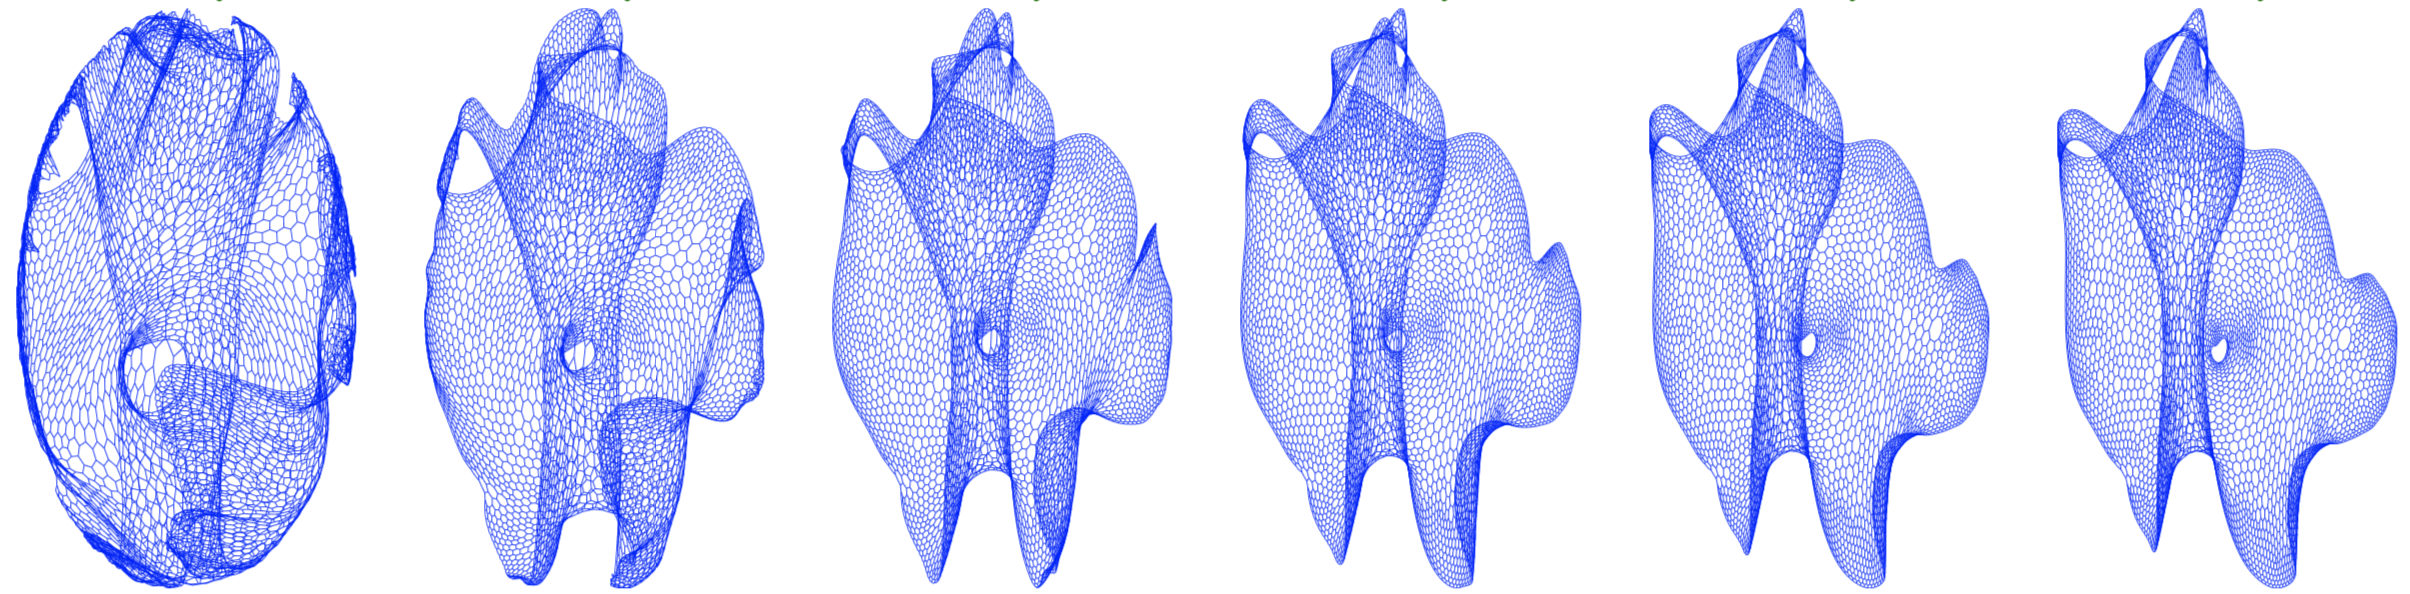
\includegraphics[height=2.2cm,width=0.8\linewidth]{layouts/batches/batch256.png}}                              \\ \hline
    \textbf{BS=1024} & \multicolumn{6}{|c|}{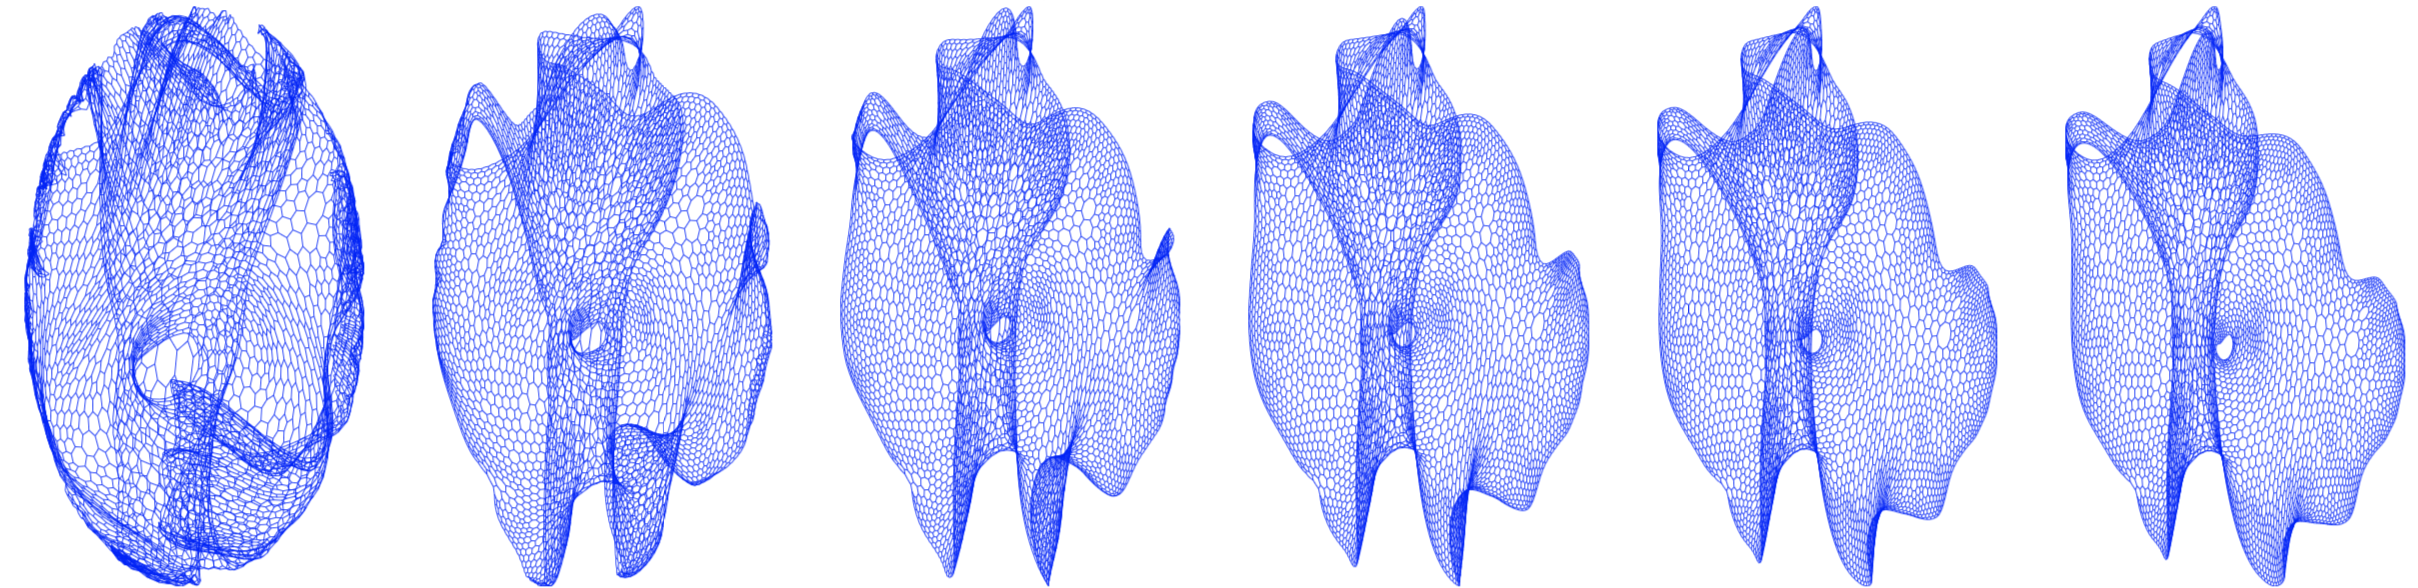
\includegraphics[height=2.2cm,width=0.8\linewidth]{layouts/batches/batch1024.png}}                              \\ \hline
    \textbf{BS=2048} & \multicolumn{6}{|c|}{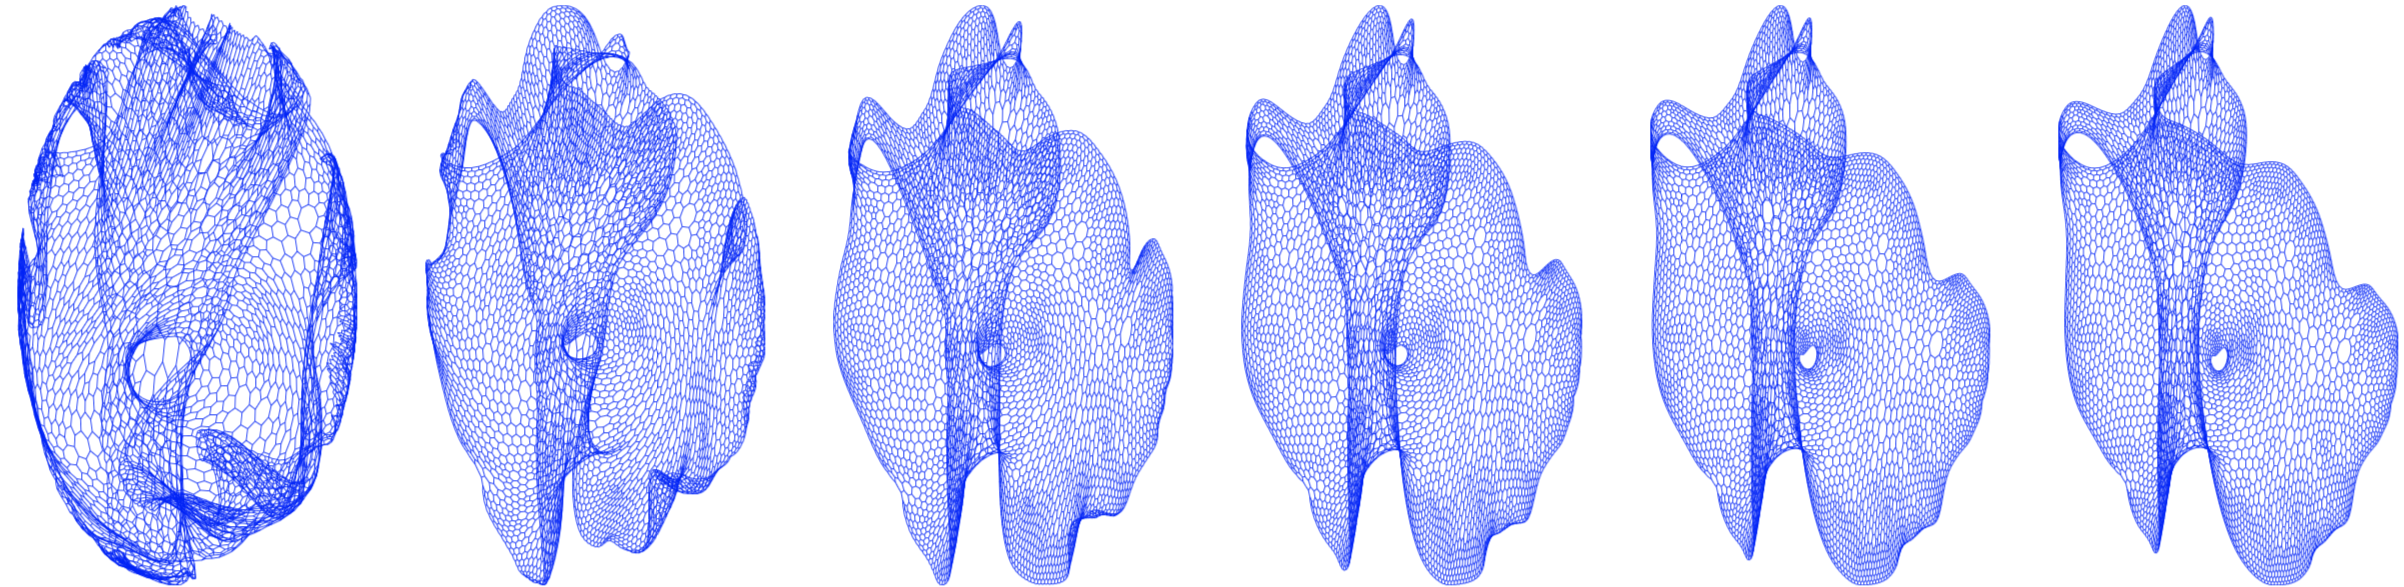
\includegraphics[height=2.2cm,width=0.8\linewidth]{layouts/batches/batch2048.png}}                              \\ \hline
            
\end{tabular}
\end{table}

\section{How to run other tools}

We have used Gephi's toolkit to run ForceAtlas2 and OpenOrd. This integrated tool is available in our repository with proper documentation. Please check out our repository for more details. We have also used OpenOrd tool from authors repository which is written in C++ language using MPI.

\noindent{}\noindent{}\noindent{}To run Gephi's ForceAtlas2, we use commands like following:

\begin{markdown}
```
java -jar othertools/GephiLayouts-1.0.jar forceatlas2 -i 3elt_dual.gml -o 3elt_dual.forceatlas2.gml -threads 8 -maxiters 600
```
\end{markdown}
\newline
\noindent{}\noindent{}\noindent{}To run Gephi's OpenOrd, we use commands like following:

\begin{markdown}
```
java -jar othertools/GephiLayouts-1.0.jar openord -i 3elt_dual.gml -o 3elt_dual.forceatlas2.gml -threads 8 -maxiters 600
```
\end{markdown}
\newline
\noindent{}\noindent{}\noindent{}To run MPI version of OpenOrd, we use commands like following:

\begin{markdown}
```
mpirun --oversubscribe -n 48 ./bin/layout ./input/3elt_dual
```
\end{markdown}
\newline
\noindent{}\noindent{}\noindent{}To run tsNET, we use commands like following:

\begin{markdown}
```
python tsnet.py 3elt_dual.vna --output 3elt_dual.out.vna --perplexity 800 --learning_rate 6000
```
\end{markdown}

\begin{table*}[t]
\caption{Running time of BatchLayout of $O(n^2)$ version for different graphs. We set number of iterations to 500 and enable \emph{-ffast-math -mavx512f -mavx512dq} flags which are available in our Skylake server.}

\centering
\begin{tabular}{|c|c|c|c|}
\hline
\textbf{Graph} & \textbf{Runtime(sec.)} & \textbf{Graph} & \textbf{Runtime(sec.)} \\ \hline

Powergrid &	0.86	 &	add32 &	0.88	\\ \hline
ba\_network  &	1.27 &	3elt\_dual & 2.38 \\ \hline	PGPgiantcompo &	3.27 & pkustk02 &	3.34 \\ \hline
fe\_4elt2 &	3.43	&		bodyy6 &	9.49 \\ \hline	pkustk01 &		12.27 &	OPF\_6000 &		22.37 \\ \hline finance256  & 34.5 &		finan512 & 131.73\\ \hline
\end{tabular}
\label{tab:measures_batchlayout_time}
\end{table*}

\begin{table*}%[t]
\caption{Running time of tsNET for different graphs. tsNET failed to run for finance256 and other graphs which have more vertices than finance256.}

\centering
\begin{tabular}{|c|c|c|c|}
\hline
\textbf{Graph} & \textbf{Runtime(sec.)} & \textbf{Graph} & \textbf{Runtime(sec.)} \\ \hline

Powergrid &	1465.63	 &	add32 &	712.68	\\ \hline
ba\_network  &	2208.14 &	3elt\_dual & 3336.54 \\ \hline	PGPgiantcompo &	7546.79 & pkustk02 &	4195.17 \\ \hline
fe\_4elt2 &	5707.4	&		bodyy6 &	26923.84 \\ \hline	pkustk01 &		26953 &	OPF\_6000 &		60557.65 \\ \hline finance256  & - &		finan512 & -\\ \hline
\end{tabular}
\label{tab:measures_tsnet_time}
\end{table*}



\begin{table*}%[t]
\caption{Comparision of Edge uniformity (EU) measures among random initialized version of \toolname{}. For this measure, lower value means better result.}

\centering
\begin{tabular}{|c|c|c|c|c|c|}
\hline
\multirow{1}{*}{\textbf{Graph}} & \multicolumn{2}{c|}{\textbf{EU}}  &  \multirow{1}{*}{\textbf{Graph}}
& \multicolumn{2}{c|}{\textbf{EU}}            \\ \cline{2-3} \cline{5-6}
                                & BLR       & BLRBH & & BLR & BLRBH  \\ \hline

Powergrid &		0.784 &		0.529 & plustk02	& 	0.844 &		0.699\\ \hline
add32 &	1.354 &		1.029 &	 fe\_4elt2 &		0.404 &		0.51\\ \hline
ba\_network	 &	1.016 &		0.566 & bodyy6 &	0.741 &		0.806 \\ \hline
3elt\_dual &		0.361 &		0.443 &	pkustk01 &	0.76 &		0.659\\ \hline
PGPgiantcompo &	0.812 &		0.704 & - &		- &	-\\ \hline

\end{tabular}
\label{tab:measures_random_init0}
\end{table*}

\begin{table*}%[t]
\caption{Comparision of Stress (ST) and Neighborhood preservation (NP) measures among random initialized version of \toolname{}. For ST, lower value means better result and for NP, higher value represents better result. }
\centering
\begin{tabular}{|c|c|c|c|c|}
\hline
\multirow{1}{*}{\textbf{Graph}} & \multicolumn{2}{c|}{\textbf{ST}}                            & \multicolumn{2}{c|}{\textbf{NP}}            \\ \cline{2-5} 
                                & BLR       & BLRBH & BLR & BLRBH  \\ \hline

Powergrid	&	1.7E+6	&	2.2E+6	&	0.336 &		0.208\\ \hline
add32	&	2.0E+6	&	2.7E+6	&	0.437	&	0.229\\ \hline
ba\_network	&	2.9E+6	&	2.8E+6	&	0.346	&	0.283\\ \hline
3elt\_dual	&	1.0E+7 &	1.3E+7	&	0.168	&	0.112\\ \hline
PGPgiantcompo	&	8.1E+6 &		1.7E+7	&	0.182	&	0.109\\ \hline
plustk02	&	2.7E+7	&	4.7E+7	&	0.412	&	0.211\\ \hline
fe\_4elt2	&	1.6E+7	&	2.1E+7	&	0.268	&	0.165\\ \hline
bodyy6	&	3.9E+7	&	4.2E+7	&	0.171	&	0.177\\ \hline
pkustk01	&	4.6E+6	&	4.2E+6	&	0.626	&	0.599\\ \hline


\end{tabular}
\label{tab:measures_random_init}
\end{table*}

\begin{figure}
    \centering
    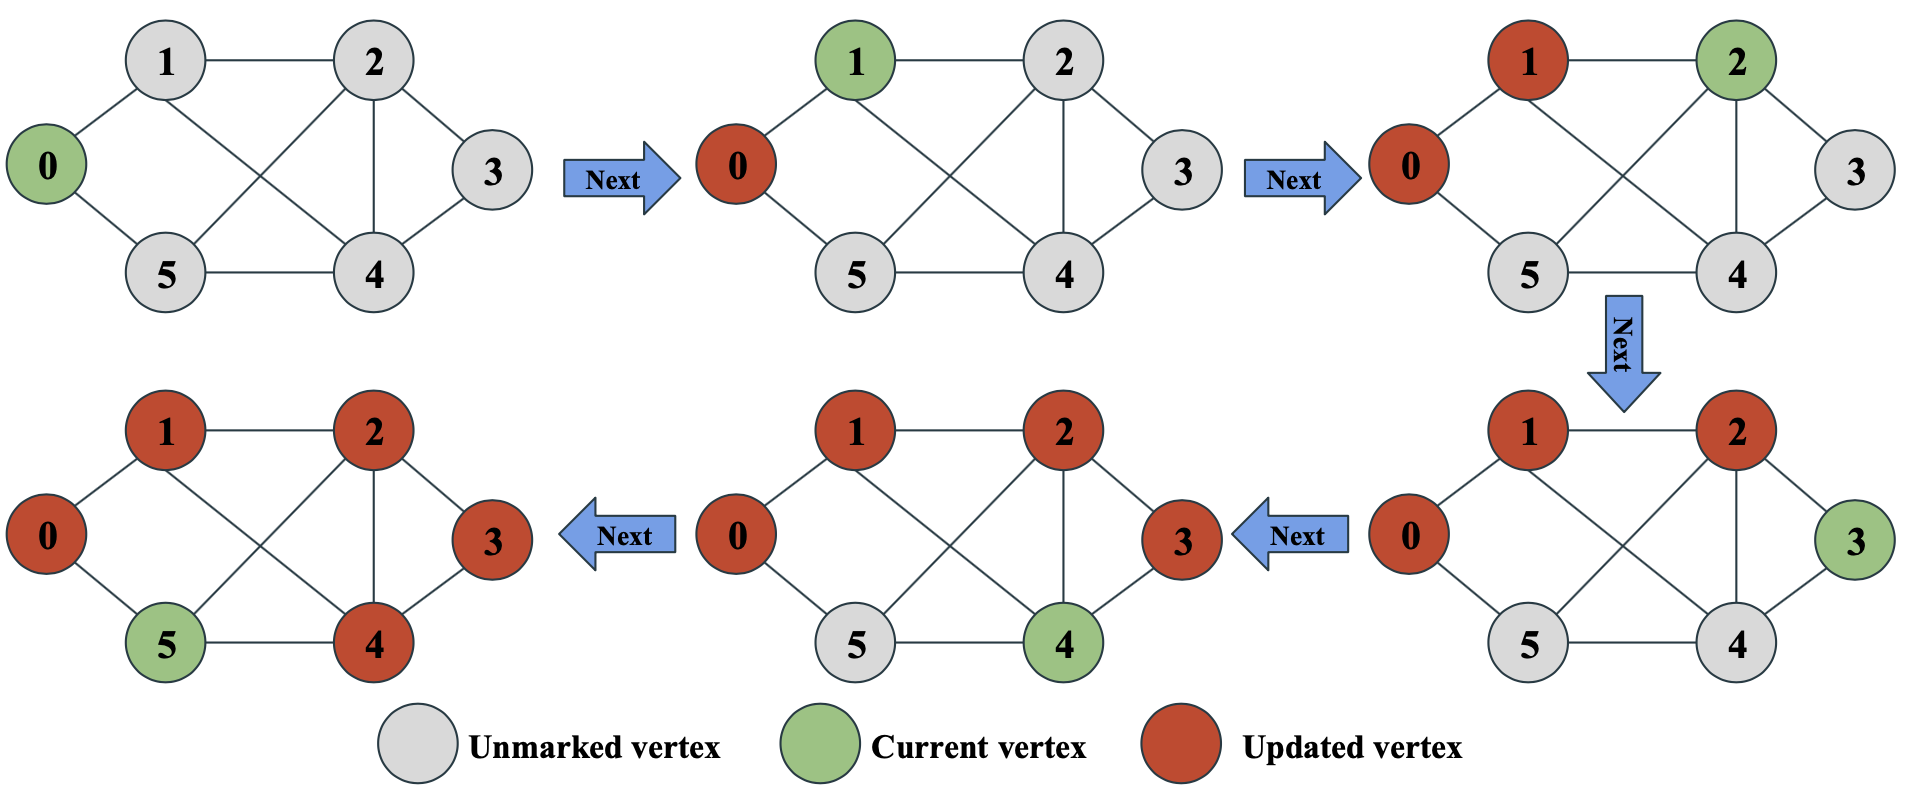
\includegraphics[width=\linewidth]{figures/sgd.png}
    \caption{Example of force calculations in sequential approach. Gray colored vertex represents unmarked vertex whose updated position has neither been calculated nor is being calculated. Green colored vertex represents current vertex whose forces are being calculated with respect to all other vertices. Red colored vertex represents those cases whose forces have already been updated/calculated.}
    \label{fig:sgdfig}
\end{figure}

\begin{figure*}
    \centering
    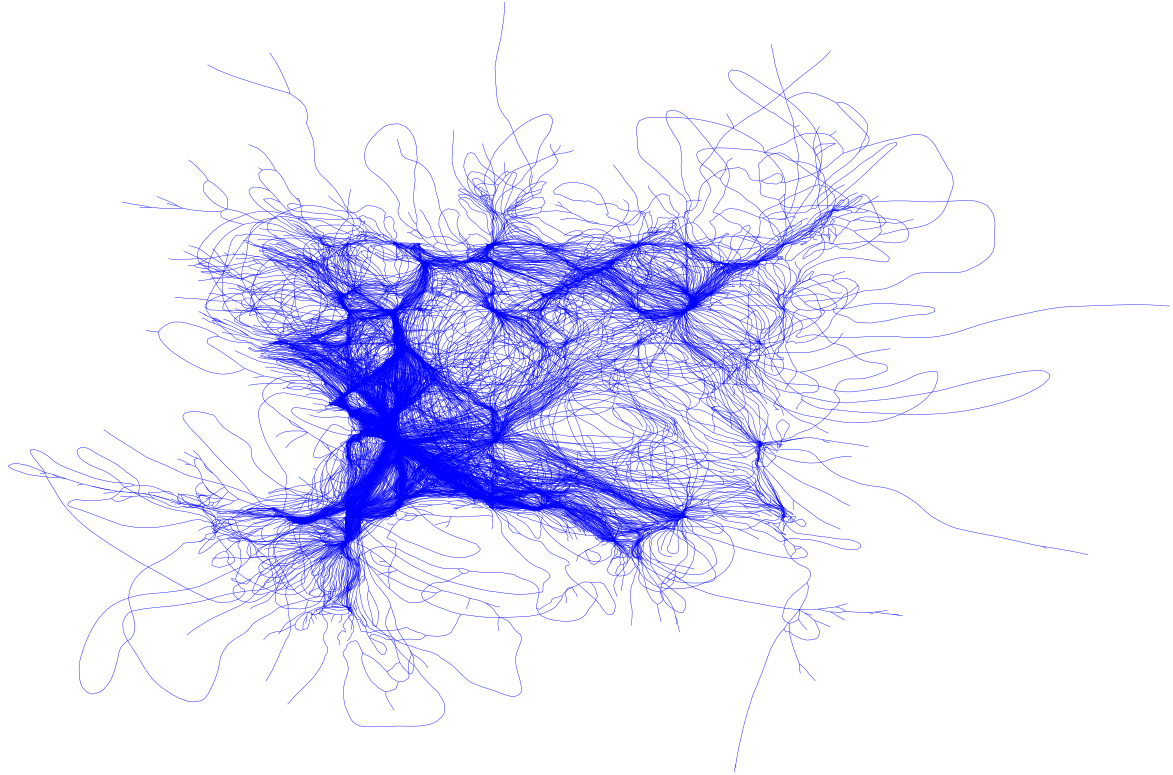
\includegraphics[width=0.32\linewidth]{layouts/BLBHlx750.png}
    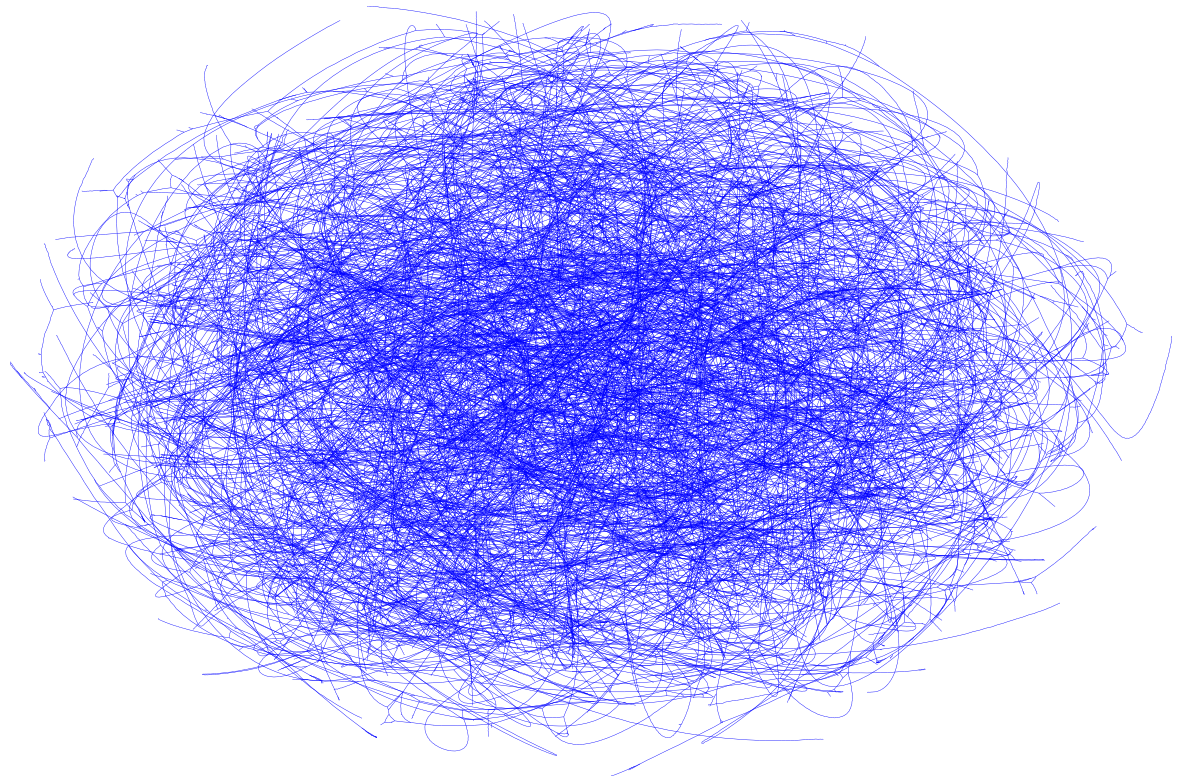
\includegraphics[width=0.32\linewidth]{layouts/FA2BHlx750.png}
    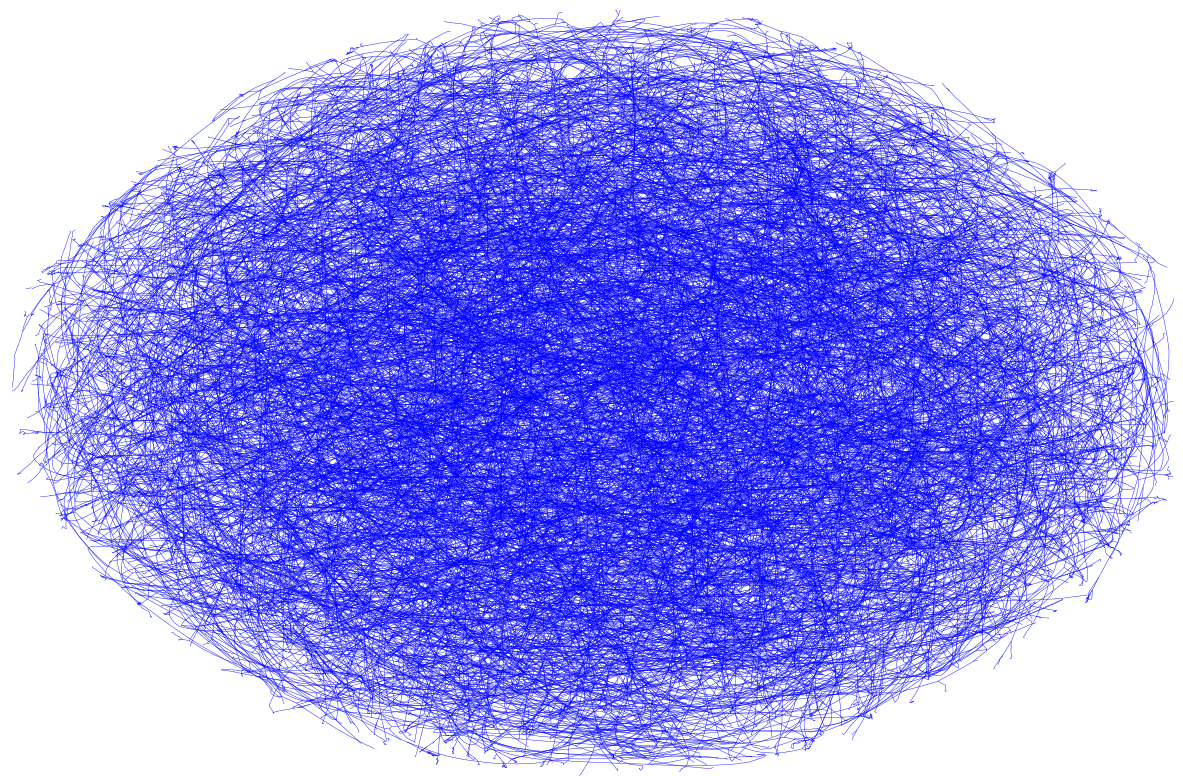
\includegraphics[width=0.32\linewidth]{layouts/OOGHoutput_lxOSM.png}
    \caption{Layouts of lxOSM which has 114,599 vertices and 239,332 edges. BatchLayoutBH (left plot), ForceAtlas2BH (middle plot) and OpenOrd (right plot) took 24.75 seconds, 102.0 seconds and 50.03 seconds, respectively for 750 iterations using 48 threads. \toolnameBH{} is capable of generating readable layout within very short time than other two tools.}
    \label{fig:biggraphs}
\end{figure*}

\begin{figure*}
    \centering
    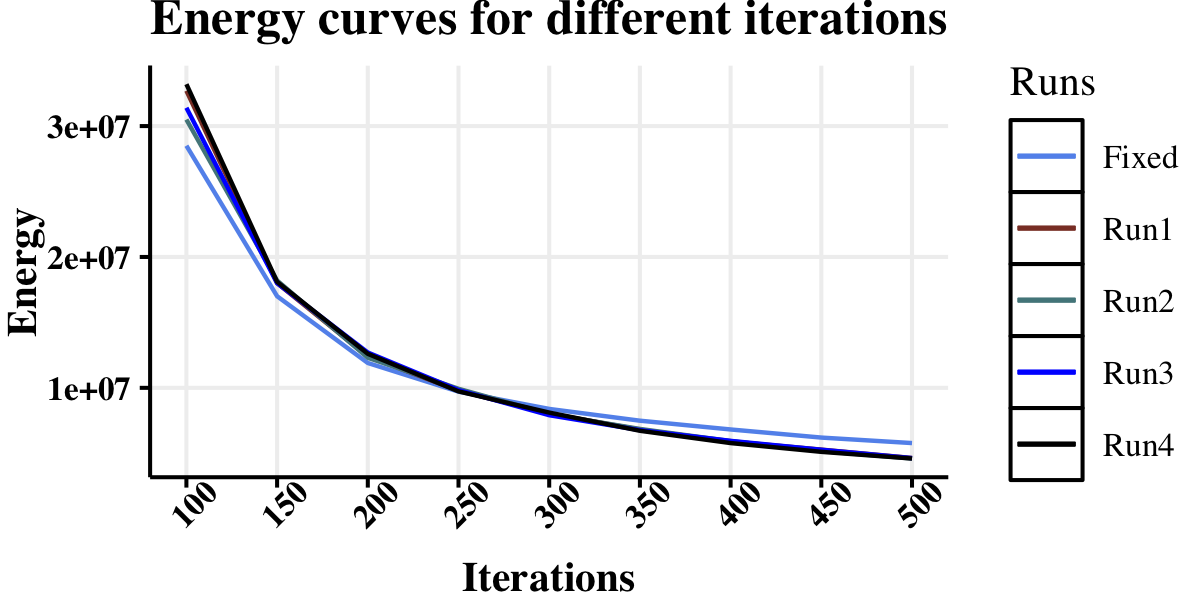
\includegraphics[width=0.48\linewidth]{figures/origrandombatches.png}
     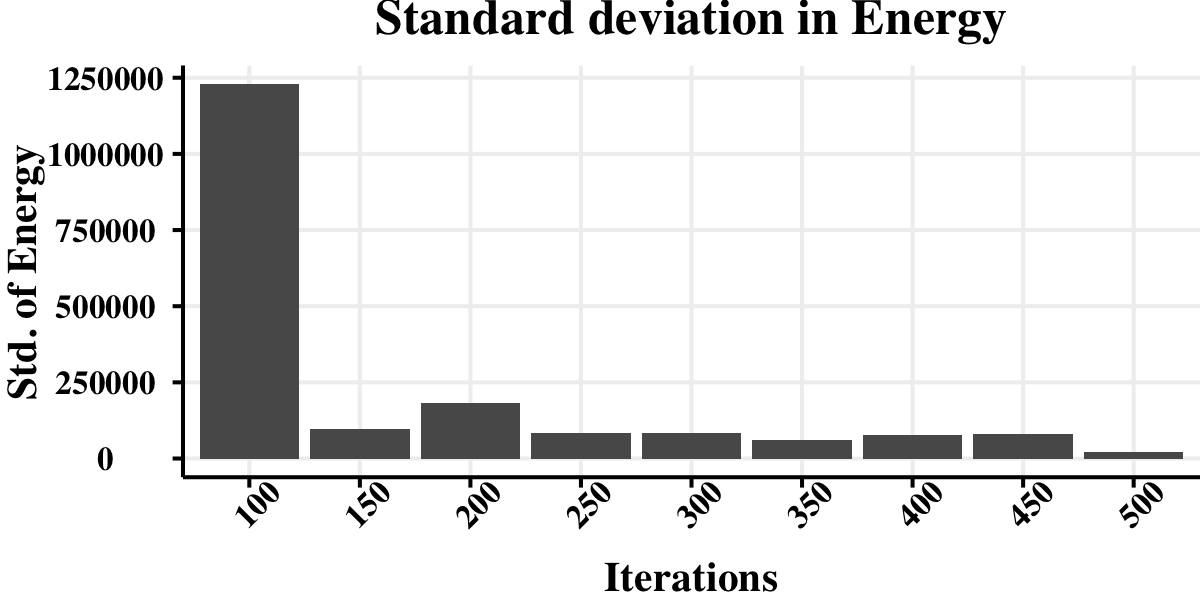
\includegraphics[width=0.48\linewidth]{figures/boxrandombatches.png}
    \caption{Energy curves of random batch selection for different runs with same hyper-parameters (3elt\_dual graph) (left figure). There are differences but due to high value of energy, it is not clearly visible and we demonstrate this difference in right figure.}
    \label{fig:origruns}
\end{figure*}


\begin{figure}
    \centering
    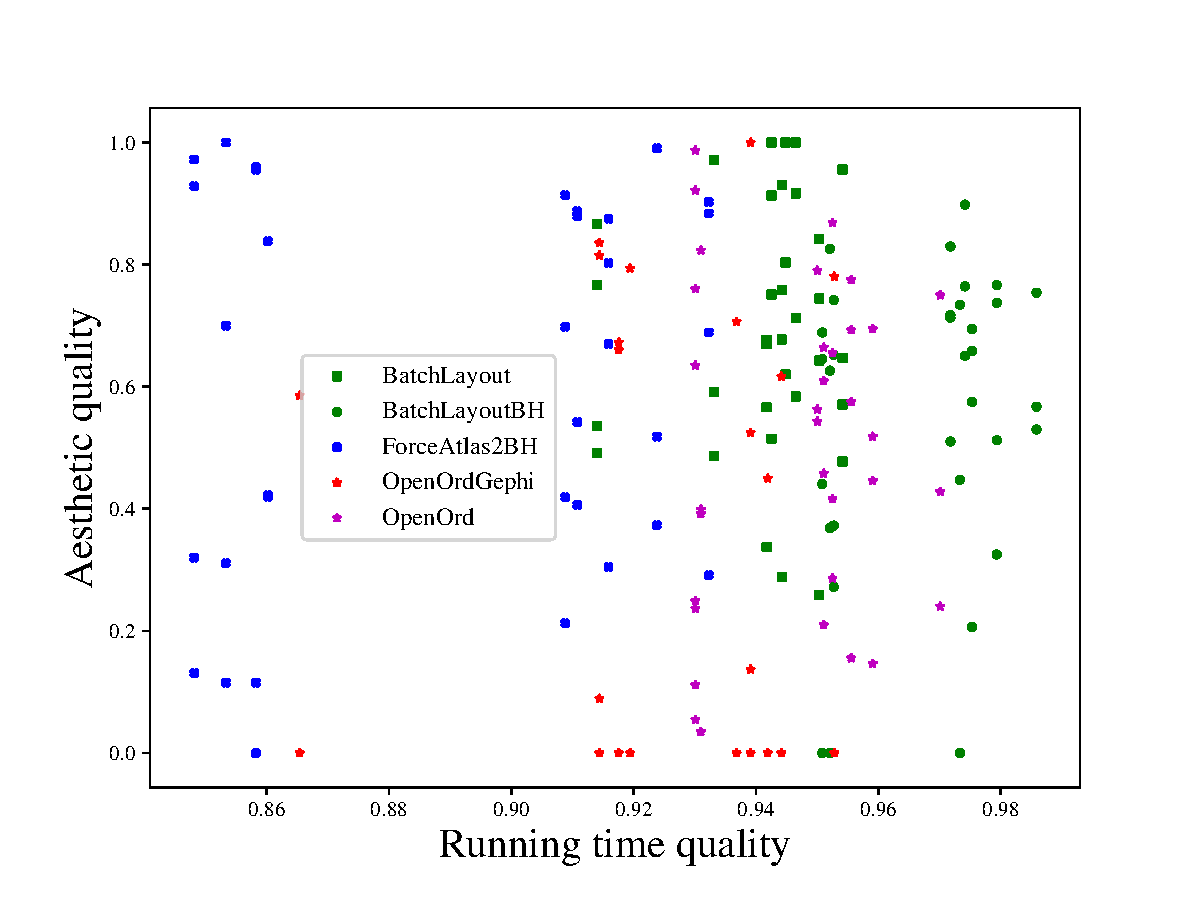
\includegraphics[width=0.7\linewidth]{figures/summary50iterations.pdf}
    \caption{Summary of running time and aesthetic quality of all tools for 500 iterations discussed in the manuscript, Tables II, III and IV. We normalize running time by dividing the maximum running time among all tools for a corresponding graph and subtracting from 1 to feel like higher number is better for quality. We similarly compute other normalized aesthetic measure to set within range 0 to 1 where higher value means better quality. We put normalized running time quality in x-axis and normalized aesthetic measures in y-axis for each corresponding graph. ForceAtlas2 is not shown due to its lower normalized value for running time which is always 0. Obviously, the best tool will touch the right-top corner i.e., better running time as well as better quality. BatchLayout and BatchLayoutBH are shown in same color to distinguish from other tools. We clearly see that BatchLayout and BatchLayoutBH attain better running time and quality.}
    \label{fig:summary500iterations}
\end{figure}

\begin{algorithm}
\caption{constructBHT}
\hspace*{\algorithmicindent} \textbf{Input:} $c$, $D$
\begin{algorithmic}[1]
\State $p_1 \leftarrow$ consecutive $c_i$'s in left top cell
\State $p_2 \leftarrow$ consecutive $c_i$'s in right top cell
\State $p_3 \leftarrow$ consecutive $c_i$'s in left bottom cell
\State $p_4 \leftarrow$ consecutive $c_i$'s in right bottom cell
\State compute diameter $D = \frac{D}{2}$
\State $t_1 \leftarrow$ constructBHT($p_1$, $D$) in parallel
\State $t_2 \leftarrow$ constructBHT($p_2$, $D$) in parallel
\State $t_3 \leftarrow$ constructBHT($p_3$, $D$) in parallel
\State $t_4 \leftarrow$ constructBHT($p_4$, $D$) in parallel
\State check coordinates if any of $t_i$'s is leaf node
\State compute centroid $s$ using $t_1$,$t_2$,$t_3$,and $t_4$
\newline
\Return create tree \emph{node} using $t_1$,$t_2$,$t_3$,$t_4$, $s$, and $D$
\end{algorithmic}
\label{algo:constructbht}
\end{algorithm}


\begin{algorithm}
\caption{calcRepulsiveForce}
\hspace*{\algorithmicindent} \textbf{Input:} $r$, $i$, $f$
\begin{algorithmic}[1]
\State $d = \parallel r_c - i\parallel$ \Comment{Euclidean distance}
\If{$\theta > \frac{D}{d}$} \Comment{MAC condition}
\State $f += f_a(r_c,i)\times \frac{r_c-i}{d}$ \Comment{$r_c$ indicates coordinates of $r$}
\Else 
\For{$child$ of $r$}
\If{$child$ has descendent}
\State calcRepulsiveForce($child$, $i$, $f$)
\Else
\State $f += f_r(child_c,i)\times \frac{child_c-i}{d}$ \Comment{$child_c$ indicates coordinates of $child$}
\EndIf
\EndFor
\EndIf
\end{algorithmic}
\label{algo:queryserve}
\end{algorithm}


\begin{algorithm}
\caption{BatchLayoutBH}
\hspace*{\algorithmicindent} \textbf{Input:} G(c, V, E)
\begin{algorithmic}[1]
\State $Step = 1.0$ \Comment{initial step length}
\State $Loop = 0$
\While {$ Loop < MaxIteration$}
\State $Energy = 0$
\State re-scale $c$ in bounding box
\State sort $c$ in parallel based on morton order
\State $D = max(max(c_x)-min(c_x),max(c_y)-min(c_y))$
\State $BHT = constructBHT(c, D)$ \Comment{call Algorithm \ref{algo:constructbht}}
\ParFor{$i \in V$}
			\State $ct_{i} = 0$
\EndParFor
\For{$b \leftarrow$ 0 to $\frac{n}{BS}-1$}
    \ParFor{$i \leftarrow b * BS$ to $(b + 1) * BS-1$ \textbf{by} $bx$}
        \State $f = (0,0)$
        \For{$j\in G.colids[i]$}
                    \State $f\;+= f_a(i,j)\times \frac{c_j - c_i}{||c_i - c_j||}$
        \EndFor 
        \State $calcRepulsiveForce(BHT, i, rf = (0,0))$ \Comment{call Algorithm \ref{algo:queryserve}}
        \State $f = f - rf$;
        \State $ct_{i+x} += f$
    \EndParFor
    \ParFor{$i \leftarrow b * BS $ to $(b + 1) * BS - 1$}
        \State $c_i\; += Step \times \frac{ct_i}{||ct_i||}$
        \State $Energy\; += ||ct_i||^2$
    \EndParFor
\EndFor
\EndWhile
\newline
\Return the final layout $c$
\end{algorithmic}
\label{algo:cbBatchLayout}
\end{algorithm}



\begin{figure}
    \centering
    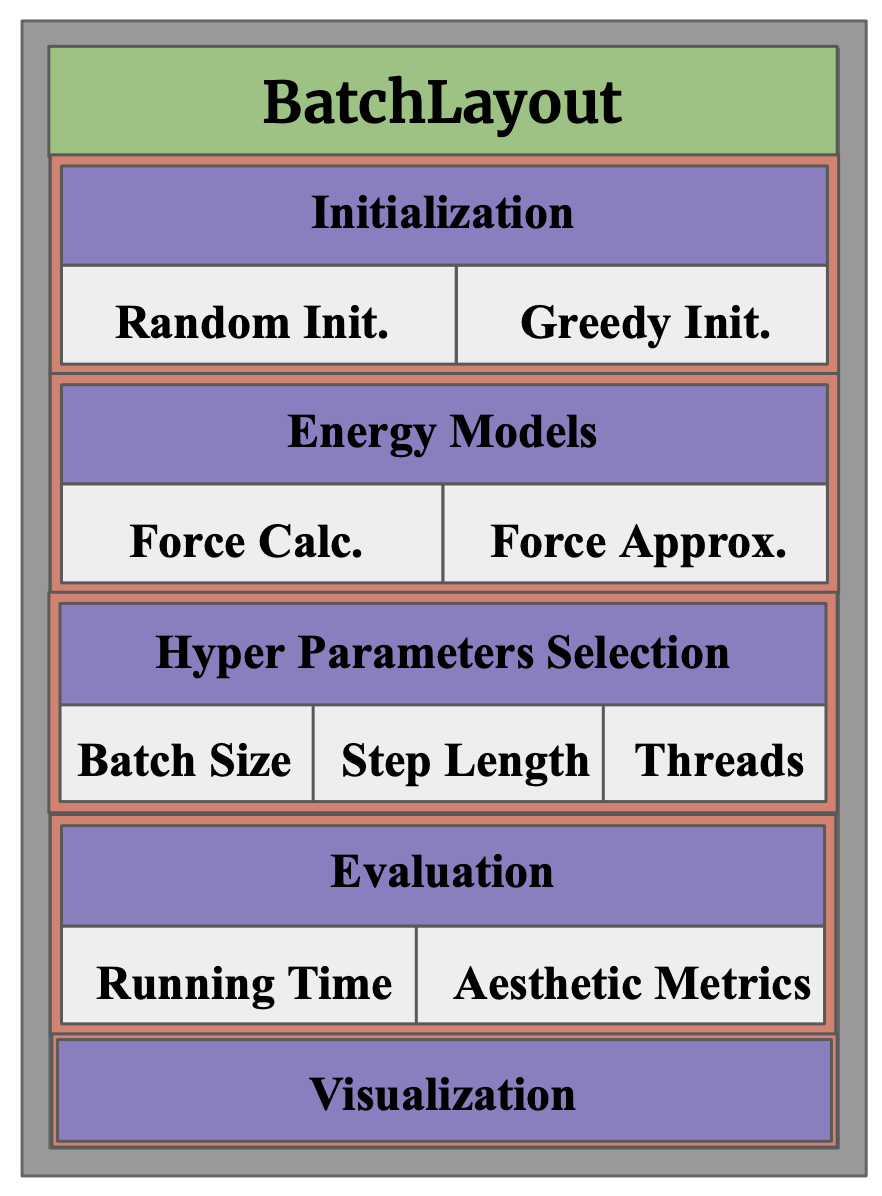
\includegraphics[width=0.3\linewidth]{figures/batchlayoutsystem.png}
    \caption{BatchLayout system overview. In BatchLayout, we demonstrate two initialization techniques, several energy models and repulsive force approximation techniques, flexibility of choosing batch size and number of threads, evaluation based on run time and aesthetic metrics, and visualization.}
    \label{fig:blsystem}
\end{figure}


\begin{table*}[t]
\caption{Running time of $FM^3$ of OGDF library for different graphs. We run default option of $FM^3$ by setting number of iterations to 500.}

\centering
\begin{tabular}{|c|c|c|c|}
\hline
\textbf{Graph} & \textbf{Runtime(sec.)} & \textbf{Graph} & \textbf{Runtime(sec.)} \\ \hline

Powergrid &	2.21	 &	add32 &	1.34	\\ \hline
ba\_network  &	2.45 &	3elt\_dual & 3.77 \\ \hline	PGPgiantcompo &	5.90 & pkustk02 &	5.27 \\ \hline
fe\_4elt2 &	4.13	&		bodyy6 &	7.75 \\ \hline	pkustk01 &		9.82 &	OPF\_6000 &		11.68 \\ \hline finance256  & 13.33 &		finan512 & 27.89\\ \hline
comYout.  & 897.17 &		Flan\_1565 & 1105.33\\ \hline
\end{tabular}
\label{tab:measures_fm3_time}
\end{table*}

\begin{table*}[]
\caption{Number of edge crossing in the layouts after running each tool for 500 iterations.}
\centering
\begin{tabular}{|c|c|c|c|c|c|}
\hline
\textbf{Graph} & \textbf{BL} & \textbf{BLBH} & \textbf{FA2} & \textbf{FA2BH} & \textbf{OO} \\ \hline
Powergrid      & 3892        & 8030          & 3300         & 3308           & 6631        \\ \hline
add32          & 5745        & 22466         & 1325         & 1608           & 17145       \\ \hline
ba\_network    & 526         & 7518          & 273          & 334            & 588         \\ \hline
3elt\_dual     & 6208        & 12678         & 13992        & 8385           & 24990       \\ \hline
PGPgiant.      & 909233      & 2096136       & 626802       & 632239         & 722747      \\ \hline
fe\_4elt2      & 51472       & 252197        & 67624        & 73995          & 133574      \\ \hline
bodyy6         & 208077      & 363718        & 153062       & 181133         & 475689      \\ \hline
\end{tabular}
\end{table*}

\end{document}